%  \documentclass[DIV=12, a4]{scrartcl}
% \documentclass[10pt, a5paper]{scrreprt}
\documentclass[a4]{scrreprt}

\usepackage[
fancytheorems, 
fancyproofs,
noindent, 
%spacingfix, 
]{adam}

% \documentclass[a4paper]{report}
% \usepackage[
% % fancytheorems, 
% noindent, 
% %spacingfix, 
% %noheader
% ]{vanilla}



% \usepackage[margin=0.75in]{geometry}

\usepackage{tikz}

% \setcounter{section}{-1}

\title{Groups}
% \subtitle{Adam Kelly}
\author{Adam Kelly}
\date{Updated \today}

\begin{document}

\maketitle

\begin{abstract}
	This set of notes is a work-in-progress account of the course `Groups', originally lectured by Dr. Ana Khukhro in Michaelmas 2020 at Cambridge. These notes are not a transcription of the lectures, but they do roughly follow what was lectured (in content and in structure).

	These notes are my own view of what was taught, and should be somewhat of a superset of what was actually taught. I frequently provide different explanations, proofs, examples, and so on in areas where I feel they are helpful. Because of this, this work is likely to contain errors, which you may assume are my own. If you spot any or have any other feedback, I can be contacted at \href{mailto:ak2316@cam.ac.uk}{ak2316@cam.ac.uk}.
\end{abstract}

\tableofcontents

\clearpage


\chapter{Groups}

`Groups' is a course which introduces you to the subject of \emph{Abstract Algebra}.
Indeed, while groups are one of the simplest and most basic of all the algebraic structures\footnote{Apart from `magmas' I suppose, but they don't tend to be a particularly useful notion.}, they are immensely useful and appear in almost every area of mathematics. 

\section{Definition of a Group}

We will begin our study of the subject by defining formally what a group is.

\begin{definition}[Group]
	A \vocab{group} is a set $G$ with a binary operation\footnote{Some texts include an additional \emph{closure} axiom, but this is implied by $*$ being a binary operation on $G$.} $*$ which satisfies the axioms:
	\begin{itemize}
		\item \emph{Identity}. There is an element $e \in G$ such that $g * e = e * g = g$ for every $g \in G$.
		\item \emph{Inverses}. For every element $g \in G$, there is an element $g^{-1} \in G$ such that $g * g^{-1} = g^{-1} * g = e$.
		\item \emph{Associativity}. The operation $*$ is associative.
	\end{itemize}
\end{definition}

We typically refer to a group as defined above by $(G, *)$, which explicitly states that $*$ is the group operation. When the operation being used is clear, we can refer to the group by just $G$. We will also be omitting the group's operation symbol quite often, for example writing $gh = g * h$. 

 In a later section, we will look at some non-trivial examples of groups.

\subsection{Elementary Properties of Groups}

With the notion of a group now defined, we can now consider some basic facts that follow directly from the definition of a group. We will first address whether it is possible for a group to have multiple identity elements, or for an element to have multiple inverses (no).

\begin{proposition}[Uniqueness of the Identity and Inverse]
	Let $(G, *)$ be a group. Then there is a unique identity element, and for every $g \in G$, $g^{-1}$ is unique.
\end{proposition}
\begin{proof}
	To prove that the identity element is unique, let $e$ and $e'$ be identity elements of $G$. Then $e* e' = e$ and $e* e' = e'$ by definition, giving $e = e'$. 
	
	To prove that the inverses are unique, suppose that for some $g, h, k \in G$ we have $g* h = g *k = e$. Then $g^{-1}* g *h = g^{-1} *g * k$, implying $h = k$. The case of $h * g = k * g = e$ follows analogously.
\end{proof}

The next useful fact is the \emph{cancellation law}, whose proof bears a large resemblance to the proof that inverses are unique.

\begin{proposition}[Cancellation Law]
	If $(G, *)$ is a group, and $a, b, c \in G$, then $a*b = a*c$ and $b*a = c*a$ both imply $b = c$.
\end{proposition}
\begin{proof}
	Taking $a * b = a * c$ and left-multiplying by $a^{-1}$ we have $a^{-1} * a * b = a^{-1} * a * c$, that is, $b = c$. The other case follows analogously.
\end{proof}

The last proposition we will prove in this section gives us a useful result about computing inverses.

\begin{proposition}[Computing Inverses]
	Let $(G, *)$ be a group, and let $g, h \in G$. Then the following hold:
	\begin{enumerate}[label=(\roman*)]
		\item $(g*h)^{-1} = h^{-1} * g^{-1}$.
		\item $(g^{-1})^{-1} = g$.
	\end{enumerate}
\end{proposition}
\begin{proof}$ $\phantom{\qedhere}
	\begin{enumerate}[label=(\roman*)]
		\item We have $(g*h) * (h^{-1} * g^{-1}) =  g * (h * h^{-1}) * g^{-1} = g * g^{-1} = e$, so $(g*h)^{-1} = h^{-1} * g^{-1}$.
		\item Similarly, $g^{-1} * g = e$, so $(g^{-1})^{-1} = g$. \hfill \qedsymbol
	\end{enumerate}
\end{proof}

\subsection{Examples of Groups}

It's probably of some use to have concrete examples of groups in your head, so you can get a feel for what they are. In this section we will present some non-trivial examples of groups (and some examples of non-groups).

It should be recognized that commutativity is \emph{not} a group axiom, and the majority of groups are not commutative. We do have a name for groups where the binary operation is commutative though.

\begin{definition}[Abelian Groups]
	We say a group $(G, *)$ is \vocab{abelian} if $*$ is commutative, that is, if for any $g, h \in G$, $g * h = h * g$.
\end{definition}

In this section, we will consider examples of both abelian and non-abelian groups\footnote{If you are not familiar with some of the concepts used, such as matrices or modular arithmetic, feel free to ignore those examples.}. In the first few cases, the reasons why they are a group are stated. For the others, you should consider how they satisfy the group axioms yourself. 

\begin{example}[The Trivial Group]
	The \vocab{trivial group} is a group whose only element is the identity, $\{ e \}$.
\end{example}

\begin{example}[Additive Group of Integers]
	$(\Z, +)$ is an group. We have
	\begin{itemize}
		\item The identity element $0 \in Z$, as $a + 0 = 0 + a = a$ for any $a \in \Z$
		\item The inverse of $a \in \Z$ being $-a$, as $a + (-a) = (-a) + a = 0$. 
		\item The operation $+$ is associative and commutative.
	\end{itemize}
\end{example}
We also have the additive group of rationals $(\Q, +)$, of reals $(\R, +)$, and of complex numbers $(\C, +)$ for the same reasons.

\begin{example}[Addition Modulo $n$]
	Let $n \in \N$, and let $\Z/n \Z = \{0, 1, \dots, n - 1\}$ denote the set of residues modulo $n$. Then $(\Z/n\Z, +)$ is a group (where addition is done modulo $n$). We have
	\begin{itemize}
		\item The identity element is $0 \pmod{n}$, as $a + 0 \equiv 0 + a \equiv a \pmod{n}$.
		\item The inverse of $a \in \Z/n\Z$ is $-a$, as $a + (-a) \equiv 0 \pmod{n}$.
		\item Addition modulo $n$ is associative.
	\end{itemize}
\end{example}

\begin{example}[Non-Zero Rationals]
	Let $\Q^\times$ denote the set of non-zero rationals. Then $(\Q^\times, \times)$ is a group.
\end{example}
Similarly, we also have the groups $(\R^\times, \times)$ and $(\C^\times, \times)$.

\begin{example}[Multiplication Modulo $p$]
	Let $p$ be a prime, and let $(\Z / p \Z)^\times$ denote the set of non-zero residues modulo $p$. Then $((\Z / p \Z)^\times, \times)$ is a group (where multiplication is done modulo $p$).
\end{example}

\begin{example}[General Linear Group]
	Let $\GL_n(\R)$ be the set of $n \times n$ matrices with non-zero determinant. Then $(\GL_n(\R), \times)$ is the \vocab{general linear group}\footnote{Using matrix multiplication}.
\end{example}

\begin{example}[Special Linear Group]
	Let $\SL_n(\R)$ be the set of $n \times n$ matrices with determinant 1. Then $(\SL_n(\R), \times)$ is the \vocab{special linear group}.
\end{example}

\subsection*{Non-Examples of Groups}

We will now give some examples of sets with operations that are not groups. It should be useful to think about why each example does not satisfy the group axioms.

\begin{example}[Non-Examples of Groups]
	The following are are all \emph{not} groups.
	\begin{itemize}
		\item $(\Z, \times)$
		\item $(\Q, \times)$
		\item The set of $2\times 2$ matrices with matrix multiplication.
		\item $(\R, *)$ where $r  * s = r\times r \times s$
		\item $(\N, *)$ where $n * m = |n - m|$.
	\end{itemize}
\end{example}

\section{Subgroups}

Given any mathematical structure, it can be useful to know about its \emph{substructure}. In the case of a group $(G, *)$, one might ask the question is there some subset $H \subseteq G$ that still acts like a group? This motivates the introduction of \emph{subgroups}.

\begin{definition}[Subgroups]
	Let $(G, *)$ be a group. A subset $H \subseteq G$ is a \vocab{subgroup} of $G$ if $(H, *)$ is also a group. If $H$ is a subgroup of $G$, we will write $H \leq G$.
\end{definition}

\begin{example}[Examples of Subgroups]
	The following are subgroups.
	\begin{itemize}
		\item For any group $G$, we have the \vocab{trivial subgroups} $\{ e \} \leq G$ and $G \leq G$.
		\item $\Z \leq \Q \leq \R \leq \C$ with addition.
		\item $\{ 0, 2, 4, \dots \} \leq \Z$ with addition.
		\item $\SL_n(\R) \leq \GL_n(\R)$ with matrix multiplication.
	\end{itemize}
\end{example}


Checking whether something is a subgroup is easier than checking if something is a group, since we already know about the structure of the group. To check whether $H$ is a subgroup of $(G, *)$, we can just check the following hold:
\begin{itemize}
	\item \emph{Closure}. $*$ is closed in $H$.
	\item \emph{Identity}. $e \in H$.
	\item \emph{Inverses}. For $h \in H$, we also have $h^{-1} \in H$. 
\end{itemize}

These can all be combined into a single test, that is sometimes known as the `subgroup checking lemma'.

\begin{lemma}[Subgroup Criterion]
	A subset $H$ of a set $G$ is a subgroup of $(G, *)$ if and only if $H$ is non-empty and $x * y^{-1} \in H$ for all $x, y \in H$.
\end{lemma}
\begin{proof}[Proof Sketch]
	First check that the conditions of $H$ being non-empty and $x * y^{-1} \in H$ imply that it's a subgroup. Then, show that if $H$ is not a subgroup, then either $H$ is empty or $x * y^{-1} \not\in H$ for some $x, y \in H$.
\end{proof}

As an example of using subgroups, let's try to characterize all of the subgroups of $(\Z, +)$.

\begin{theorem}[Subgroups of $\Z$]\label{thm:subgroups-of-z}
	The subgroups of $(\Z, +)$ are precisely the subsets of the form $n \Z$ for $n \in N$, where $n\Z = \{n k \; : \; k \in \Z\}$.
\end{theorem}
\begin{proof}
	First, we prove that $n \Z$ is a subgroup. Fix $n \in \N$.
	\begin{itemize}
		\item \emph{Closure}. Given $n k_{1}, n k_{2} \in n \Z,$ then $n k_{1}+n k_{2}=n\left(k_{1}+k_{2}\right) \in n \Z$.
		\item \emph{Identity}. $0 =n \cdot 0 \in n \Z$.
		\item \emph{Inverses}. The inverse of $n k$ is $-n k=n(-k) \in n \Z$.
	\end{itemize}
Thus each is subgroup. Now we prove that there is no other subgroups.

Let $H \leq Z$. If $H=\{0\}$, then $H \equiv 0 \Z$. If not, then take the smallest positive element in $H$ (namely $n$ ). since $H$ is a subgroup, it's closed and contains inverses, so $n+n+\cdots+n \in$ $H$ and $-n-n-n-\cdots-n \in H,$ so $n \Z \subseteq H$.

Suppose, for a contradiction, there is some $k \in H$ such that $k \neq n \Z .$ So, there is some integer $n$ such that $n m<k<n(m+1) .$ But then $0 \leq k-n m<n,$ and $k-n m \in H$ which is a contradiction, so $H=n \Z$.
\end{proof}

We can use the definition of a subgroup to prove some elementary facts.
\begin{proposition}[Elementary Properties of Subgroups]
	Let $G$ be a group.
	\begin{enumerate}[label=(\roman*)]
		\item Let $H$ and $K$ be subgroups of $G$. Then $H \cap K \leq G$.
		\item If $K \leq H$ and $H \leq G$ then $K \leq G$ (being a subgroup is transitive).
		\item If $K \subset H$, $H \leq G$ and $K \leq G$, then $K \leq H$. 
	\end{enumerate}
\end{proposition}
\begin{proof} There is multiple ways to prove these, but we will use the subgroup criterion as an example of it being used.\phantom{\qedhere}
	\begin{enumerate}[label=(\roman*)]
		\item Note that $H \cap K$ is not empty as $e \in H$ and $e \in K$. Then, for any $x, y \in H \cap K$, it suffices to show that $x * y^{-1} \in H$. By the subgroup criterion, we have $x * y^{-1} \in H$ and $x*y^{-1} \in K$, thus $x * y^{-1} \in H \cap K$, and we are done.
		\item If $K \leq H$, then for any $x, y \in K$, we have $x * y^{-1} \in K$. Then as $K \subset H \subset G$, we must have $x * y^{-1} \in G$, and thus $K \leq H$.
		\item As $K \leq G$, we know $K$ is non-empty. Thus it suffices to show that $x * y^{-1} \in K$ for any $x, y \in H$. But this is implied by $K \leq G$ and the subgroup criterion, and thus as $K \subset H$, $K \leq H$. \hfill \qedsymbol
	\end{enumerate}
\end{proof}

\subsection{Generators}

We will now consider a certain kind of subgroup, which is specified by some of the elements it contains.

\begin{definition}[Subgroup Generated By A Subset]
	For some set $X \subseteq G$, we define the \vocab{subgroup generated by $X$}, $\langle X \rangle$, to be the smallest subgroup of $G$ which contains $X$.
\end{definition}

From this definition, we can see that we must have $e \in \langle X \rangle$ and $X \subseteq \langle X\rangle$. Also, $\langle X \rangle$ must contain all products of elements in $X$ and their inverses.
We can put this in a more useful form with the following proposition.

\begin{proposition}
	Let $X$ be a non-empty subset of $G$. Then $\langle X \rangle$ is the set of elements of $G$ of the form 
	$x_1^{\alpha_1} x_2^{\alpha_2} \cdots x_k^{\alpha_k}$ where $x_i \in X$ (not necessarily distinct), $\alpha_i = \pm 1$ and $k \geq 0$
	(For $k = 0$, we say the element is $e$).
\end{proposition}
\begin{proof}
	Let $T$ be the set of such elements. Clearly $T \subseteq \langle X \rangle$, and also clearly $T$ is a subgroup of $G$. We also have that $X \subseteq T$ so $\langle X \rangle \subseteq T$. Thus $T = \langle X \rangle$.
\end{proof}
  
\begin{example}
	We have $(\Z, +) = \langle 1 \rangle = \langle 2, 3 \rangle$\footnote{Note that we write $\langle 2, 3\rangle$ instead of $\langle \{2, 3\} \rangle$.}, and $\Z/5\Z = \langle 1 \rangle = \langle 3 \rangle$.
\end{example}

In the above examples, we found that there was some subset of the elements in each of the group where if we considered the subgroup generated by those elements, we get the entire group.
There is a special name for such subsets.

\begin{definition}[Generators]\label{def:generator}
	If $X$ is a subset of $G$ such that $\langle X \rangle = G$, then we call $X$ a \vocab{generating set} of $G$.
\end{definition}

Notably, these generators are not necessarily unique, as can be seen in the example above.


\section{Homomorphisms}

Imagine you had two groups, $G$ and $H$ and you wanted to think of a function from $H$ to $G$ that preserved some of the structure of the group.
Let's say the function was $\phi : H \rightarrow G$. We could take any two elements $h_1, h_2 \in H$, and we could find $h_1 h_2$, and then apply $\phi$ to get $\phi(h_1 h_2)$.
Alternatively, we could try and find $\phi(h_1)$ and $\phi(h_2)$, and then get $\phi(h_1) \phi(h_2)$. If these were the same, then the function $\phi$ would indeed preserve some of the structure of the group. This motivates the introduction of \emph{homomorphisms}.

\begin{definition}[Homomorphism]
	Let $(G, *_G)$ and $(H, *_H)$ be groups. A function $\phi : H \rightarrow G$ is a \vocab{group homomorphism} if for all $a, b \in H$,
	$$
	\phi(a *_H b) = \phi(a) *_G \phi(b).
	$$
\end{definition}

\begin{example}[Inclusion Function]
	If $H \leq G$, then the function $\iota : H \rightarrow G$ that has $\iota(h) = h$ for $h \in H$ is a homomorphism. It is also injective.
\end{example}

\begin{example}
	The function $\phi : \Z\rightarrow \Z/n\Z$ with $\phi(k) = k \pmod{n}$ is a homomorphism, since for $k, l \in \Z$,
	$$
\phi(k + l) = (k + l) \bmod{n} = (k \bmod{n}) + (l \bmod{n}) = \phi(k) + \phi(l).
	$$
	$\phi$ is also surjective, since $\{0, 1, \cdots, n - 1\}$ are all the possible residues modulo $n$.
\end{example}

\begin{example}
	The function $\phi : (\R, + )\rightarrow (\R^*, \cdot)$ where $x \rightarrow e^x$ is a homomorphism. We have
	$$
	\phi(x + y) = e^{x + y} = e^x \cdot e^y = \phi(x) \cdot \phi(y).
	$$
	It is injective, as $e^x = e^y$ implies $x = y$ using logarithms, and surjective, as given $a \in \R^*$, $\phi(\log a) = e^{\log a} = a$.
\end{example}

We can see some natural consequences of this definition of a homomorphism, which shows how well it preserves the group's structure.

\begin{proposition}[Properties of Homomorphisms]
	Let $\phi : H \rightarrow G$ be a homomorphism.
	\begin{enumerate}[label=(\roman*)]
		\item $\phi(e_h) = e_g$. 
		\item $\phi(h^{-1}) = \phi(h)^{-1}$ for all $h \in H$.
		\item If $\psi : G \rightarrow K$ is another homomorphism, then $\psi \circ \phi : H \rightarrow K$ is also a homomorphism.
	\end{enumerate}
\end{proposition}
\begin{proof}
	$ $ \phantom{\qedhere}
	\begin{enumerate}[label=(\roman*)]
		\item We have $e_H *_H e_H = e_H$, so $\phi(e_H * e_H) = \phi(e_H) *_G \phi(e_H) = \phi(e_H)$, so by the cancellation law, $\phi(e_H) = e_G$.
		\item Consider $\phi(h) *_G \phi(h^{-1}) = \phi(h *_H h^{-1}) = \phi(e_H) = e_G$, by (i). So $\phi(h) *_G = \phi(h^{-1}) = e_G$ which is the defining property of an inverse, so $\phi(h^{-1}) = \phi(h)^{-1}$.
		\item We have 
		\begin{align*}
			(\psi \circ \phi)(a *_H) &= \psi(\phi(a *_H b))\\
									 &= \psi(\phi(a) *_G \phi(b))\\ 
									 &= \psi(\phi(a)) *_K \psi(\phi(b)) \\
									 &= (\psi \circ \phi)(a) *_K (\psi \circ \phi)(b),
		\end{align*}
		so $\psi \circ \phi$ is a homomorphism from $H \rightarrow K$.\hfill \qedsymbol
	\end{enumerate}
\end{proof}


There is a special case of homomorphism, which we can use to define when two groups `are the same'.

\begin{definition}[Isomorphism]
	If a function $\phi : H \rightarrow G$ is bijection, and $\phi$ is also a homomorphism from $H \rightarrow G$, then we say it is an \vocab{isomorphism}. We say two groups $H, G$ are \vocab{isomorphic}, written $H \cong H$ if there is an isomorphism from $H \rightarrow G$.
\end{definition}

Having an isomorphism between two groups can be thought of in a few ways. Because we have a bijection function between the two groups, the groups must have the same order. But also, because a homomorphism preserves the structure of the group, we must also have the same group-structure within each group. Thus, when we have two isomorphic groups, we can think of them as two different descriptions of the same group.

For example, we might claim that `there is exactly one group of order 2', and what we mean is that for any group of order 2, we can find an isomorphism to any other group of order 2. 

\begin{example}
	Consider the group $G = \{ 1, i, -1, -i \}$ with complex multiplication. Then $G \cong \Z / 4 \Z$. This is isomorphic with the isomorphism $\phi : G \rightarrow \Z / 4 \Z$, where
	\begin{align*}
		\phi(1) &= 0, \\
		\phi(i) &= 1, \\
		\phi(-1) &= 2, \\
		\phi(-i) &= 3
	\end{align*}
	The general case is true too, where the group $H = \{  e^{2 \pi i k/n} : 0 \leq k \leq n - 1 \}$ with complex multiplication is isomorphic to $\Z /n \Z$.
\end{example}

\begin{example}[$\Z$'s subgroups are isomorphic]
	$\Z \cong n \Z$ for $n \in \Z$, as defined in \autoref{thm:subgroups-of-z}. 
\end{example}

It's worth noting that because isomorphisms are bijective, we have the following result.

\begin{proposition}[Inverses of isomorphisms are isomorphisms]
	Let $\phi : H \rightarrow G$ be an isomorphism. Then $\phi^{-1} : G \rightarrow H$ is also an isomorphism.
\end{proposition}
\begin{proof}[Proof Sketch]
	Check that $\phi^{-1}$ is a homomorphism.
\end{proof}

\subsection{Kernels}

When dealing with homomorphisms, say $\phi : H \rightarrow G$, it is useful to be able to think about what elements in $H$ our homomorphism `reaches'.
Another useful idea is thinking about what elements in $H$ get mapped to the identity of $G$. To think about these questions, we use concepts of a homomorphism's \emph{image} and \emph{kernel}. 

\begin{definition}[Image]
	Let $\phi :H \rightarrow G$ be a homomorphism. We define the \vocab{image} of $\phi$ to be the set
	$$
	\image(\phi) = \{ g \in G \; : \; g = \phi(h) \text{ for some } h \in H  \}.
	$$
\end{definition}
\begin{definition}[Kernel]
	Let $\phi : H \rightarrow G$ be a homomorphism. We define the \vocab{kernel} of $\phi$ to be the set
	$$
	\kernel(\phi) = \{ h \in H \; : \; \phi(h) = e_G \}.
	$$
\end{definition}

Indeed, while both of these are subsets of $G$ and $G$ respectively, they are also subgroups.

\begin{proposition}[The Image and Kernel are Subgroups]
	Let $H$ and $G$ be groups and let $\phi : H \rightarrow G$ be a homomorphism. Then $\image(\phi)$ is a subgroup of $G$, and $\kernel(\phi)$ is a subgroup of $H$.
\end{proposition}
\begin{proof}
	We consider the two sets separately.
	\begin{enumerate}
		\item We will show $\image(\phi) \leq G$. For any $x, y \in \image(\phi),$ let $x = \phi(x')$ and $y = \phi(y')$ for $x', y' \in H$. Then
		$$
		\phi(x' {y'}^{-1}) = \phi(x')\phi(y')^{-1} = x y^{-1} \in \image(\phi),
		$$
		thus by the subgroup criterion $\image(\phi) \leq G$.
		\item Now we show $\kernel(\phi) \leq H$. For $x, y \in \kernel(\phi)$, we have $xy^{-1} \in \kernel(\phi)$, as 
		$$
		\phi(xy^{-1}) = \phi(x)\phi(y^{-1}) = \phi(x)\phi(y)^{-1} = e_G,
		$$
		so again using the subgroup criterion, $\kernel(\phi) \leq H$. 
	\end{enumerate}
\end{proof}

\begin{example}
	$\phi : \Z \rightarrow \Z/n\Z$, where $\phi(k) = k \pmod{n}$ has $\image(\phi) = \Z/n\Z$ and $\kernel(\phi) = n\Z$.
\end{example}

One of the beauties of introducing the kernel and image is that it allows us to easily see whether a homomorphism is surjective or injective.

\begin{proposition}[Surjectivity and Injectivity Criterion]
	Let $\phi : H \rightarrow G$ be a homomorphism.
	\begin{enumerate}[label=(\roman*)]
		\item $\phi$ is surjective iff $\image(\phi) = G$.
		\item $\phi$ is injective iff $\kernel(\phi) = \{e\}$.
	\end{enumerate}	
\end{proposition}
\begin{proof}
	The first is true by definition, so we prove (ii). Suppose $\phi$ is injective, then as we have $\phi(e_H) = e_G$, so $e_H$ must be the only element sent to $e_G$ (by the definition of injectivity), which implies that $\kernel(\phi) = \{ e_H \}$.
	Now suppose that $\ker(\phi) = \{ e_h \}$. Then if $\phi(a) = \phi(b)$ for some $a, b \in H$, we  have $\phi(ab^{-1}) = \phi(a)\phi(b)^{-1} = \phi(b)\phi(b)^{-1} = e_G$. However, this implies $ab^{-1} = e_H$, so $a = b$, and $\phi$ is injective.
\end{proof}



\subsection{Direct Products}

How can we easily find a group that will have two given groups $G, H$ as subgroups?
With the aim of getting the simplest construction possible, we can `stick them together': by defining a group operation on the product $G \times H = \{ (g, h)  \; : \; g \in G, h \in H\}$ (a set of ordered pairs).

\begin{definition}[Direct Product]
	The \vocab{direct product} of two groups $G$, $H$ is the set $G \times H$ with the operation of component-wise composition,
	$$
	(g_1, h_1) * (g_2, h_2) = (g_1 *_G g_2, h_1 *_H h_2).
	$$
\end{definition}

\begin{proposition}
	The direct product of two groups $G$ and $H$ is a group.
\end{proposition}
\begin{proof}[Proof Sketch]
	Check everything component-wise.
\end{proof}

This group contains subgroups isomorphic to $G$ and $H$, taking $G \times \{ e_H \}$ and $\{ e_G \} \times H$.

A useful idea might be to try and recognize when a group is a direct product of two groups. This can be done with the following theorem.

\begin{theorem}[Direct Product Theorem]
	Let $H, K \leq G$ such that
	\begin{enumerate}[label=(\roman*)]
		\item $H \cap K = \{e\}$
		\item $\forall h \in H$ and $k \in K$, we have $hk = kh$
		\item $\forall g \in G$, there exists $h \in H$, $k \in K$ such that $g = hk$
	\end{enumerate}
	then $G \cong H \times K$.
\end{theorem}
% 
% {\color{red} TODO: Fill in details here}
\begin{proof}
	Consider the function $\phi : H \times K \rightarrow G$, where $\phi(h, k) = hk$.
	$\phi$ is a homomorphism, as
	\begin{align*}
		\phi((h_1, k_1) \cdot (h_2, k_2)) = \phi(h_1 h_2, k_1 k_2) = h_1 h_2 k_1 k_2 = h_1 k_1 h_2 k_2 = \phi(h_1, k_1) \phi(h_2, k_2).
	\end{align*}
	$\phi$ is surjective by (ii), and now we will show $\phi$ is injective.
	Suppose that $(h, k) \in \kernel\phi$. Then $h = k^{-1}$, which implies that $h, k \in H \cap K$ by (i), and thus $(h, k) = (e_H, e_K)$. Thus $\kernel \phi = \{(e_H, e_K)\}$, so $\phi$ is injective by the injectivty criterion.
\end{proof}

We now have two ways to think about the direct product. 
\begin{itemize}
	\item If we have two groups $H$, $K$, we can form their direct product $H \times K$, and view $H$ and $K$ as subgroups, namely $H \times \{e_k\}$ and $\{e_H\} \times K$.
	\item Given a group with subgroups $H$ and $K$, which satisfy the conditions of the direct product theorem, then we know that we are really dealing with $H \times K$.
\end{itemize}
Indeed these are just two descriptions of the same thing. The convention is often to refer to $H \times \{e_k\}$ and $\{e_H\} \times K$ as just $H$ and $K$ respectively.

\chapter{Important Groups}

Now that we have seen some properties of groups, we will now consider some important examples of groups.

\section{Cyclic Groups}

Recall the notion of a generator from \autoref{def:generator}.

\begin{definition}[Cyclic]
	If $G$ is a group and there is some $a \in G$ such that $\langle a \rangle = G$, then we say $G$ is \vocab{cyclic}. 
\end{definition}
Notably, if this is the case, for all $b \in G$, there exists $k \in \Z$ such that $b = a^k$.

\begin{example}[Examples of Cyclic Groups]
	The following groups are all cyclic.
	\begin{itemize}
		\item $(\Z, +)$, which is generated by $\langle 1 \rangle$ or $\langle -1 \rangle$.
		\item $(\Z/n\Z, +)$, generated by $\langle 1 \rangle$. Indeed, any $k$ coprime to $n$ will satisfy $\langle k \rangle = \Z/n\Z$.
		\item Let $G = \{ e^{2 \pi i k/n}  : 0 \leq k \leq n - 1 \}$. Then $(G, \cdot)$ is generated by $\langle e^{2 \pi i k/n}\rangle$ where $k$ is coprime to $n$.
	\end{itemize}
\end{example}
These groups all have the same `feel' to them, and indeed they are all isomorphic to the following group.

\begin{definition}[Cyclic Group $C_n$]
	Let $C_n$ be the group of elements $\{e = a^0, a, a^2, \dots, a^{n - 1}\}$, where $a^k * a^j = a^{k + j \pmod{n}}$. Then $(C_n, *)$ is the \vocab{cyclic group of order $n$}.
\end{definition}

\begin{theorem}[Cyclic Groups are Isomorphic]
	A cyclic group $G$ is isomorphic to $\Z$ or to $C_n$ for some $n \in \N$.
\end{theorem}
\begin{proof}
	As $G$ is cyclic, we have $\langle b \rangle = G$, for some $b \in G$.
	Now let's suppose that there's some $n$ such that $b^n = e$. Then define $\phi: C_n \rightarrow G$ by $\phi(a^k) = b^k$ for $0 \leq k \leq n - 1$.
	Then for any $a^j$ and $a^k \in C_n$, we trivially have that $\phi(a^j a^j) = \phi(a^{j + k}) = b^{j + k} = b^j b^k = \phi(a^j) \phi(a^k)$. Thus $\phi$ is a homomorphism.
	$\phi$ is also surjective as all elements in $G$ can be written as $b^k$, $0 \leq k < n$. It is also injective, since $\phi(a^k) = e \implies b^k = e$ and so $k = 0$ (otherwise it contradicts the minimality of $n$). So $\phi$ is an isomorphism, and $G \cong C_n$.

	If there is no such $n$, then we define $\phi : \Z \rightarrow G$ by $\phi(k) = b^k$. Then $\phi(k + m) = b^{k + m} = b^k b^m = \phi(k) \phi(m)$, so $\phi$ is a homomorphism. It is also clearly surjective.
	Now suppose $m \in \kernel(\phi)$. Then $\phi(m) = b^m = e$, and $\phi(-m) = b^{-m} = e$, so if $m \neq 0$, we would get a contradiction to the fact that there is no $n > 0$ with $b^n = e$. So $m = 0$, $\kernel(\phi) = \{0\}$ and $\phi$ must be an isomorphism. Thus $G \cong \Z$.
\end{proof}

Because of this theorem, we will often just write $C_n$ or $\Z$ for a cyclic group, regardless of its description.

\begin{proposition}
	Cyclic groups are abelian.
\end{proposition}
\begin{proof}[Proof Sketch]
	Check definitions.
\end{proof}

The idea of there being some $k$ such that $g^k = e$ for some $g$ is a frequently occuring concept.

\begin{definition}[Order of an Element]
	The \vocab{order of an element} $g \in G$ is the smallest $n \in \N$ such that $g^n = e$. This is sometimes written $\operatorname{ord}_G(g) = n$. If there is no such $n$, we say $g$ has \vocab{infinite order}.
\end{definition}

\begin{theorem}[Fundamental Theorem of Orders]
	Let $G$ be a group, and let $g \in G$ have finite order $n$. Then if $g^k = 1$, we have $n \mid k$.
\end{theorem}
\begin{proof}
	By the division algorithm, we can write $k = qn + r$ uniquely with $q, r \in \Z$ and $0 \leq r < n$. Then we have
	$$
	g^{k} = g^{qn + r} = g^{qn} g^r = (g^n)^q g^r = g^r = e.
	$$
	But we defined $n$ to be the smallest positive power for which $g^n = e$, and as $r < n$, we must have $r = 0$, otherwise we contradict the minimality of $n$. Thus $k = qn$, that is, $n \mid k$.
\end{proof}

\section{Dihedral Group}

Group theory is frequently thought of as the `algebraic study of symmetry'. With this rather vague claim in mind, we will now look at some groups related to geometry -- the symmetries of a regular $n$-gon. Let's define what we mean by a `symmetry' of a regular polygon.

\begin{definition}
	A \vocab{symmetry} of a regular $n$-gon is a transformation of the $n$-gon, so that when the transformed $n$-gon is placed on the original $n$-gon, it exactly covers it.
\end{definition}

\begin{definition}
	The \vocab{dihedral group} $D_{2n}$ is the group of symmetries of a regular $n$-gon, where the group operation is the composition of symmetries.
\end{definition}

Clearly in this group, we will have $n$ rotations (clockwise) of the angle $\frac{2 \pi k}{n}$, $0 \leq k < n$ ($k = 0$ gives the identity or `do nothing' symmetry). There is also $n$ reflections.
\begin{center}
	

\tikzset{every picture/.style={line width=0.75pt}} %set default line width to 0.75pt        

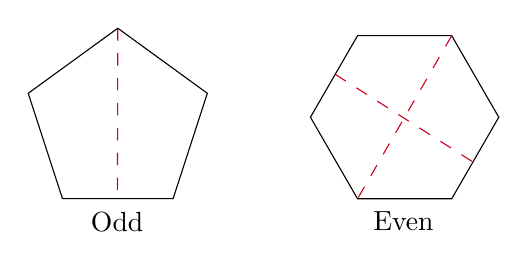
\begin{tikzpicture}[x=0.75pt,y=0.75pt,yscale=-1,xscale=1]
%uncomment if require: \path (0,300); %set diagram left start at 0, and has height of 300

%Straight Lines [id:da021745834724475888] 
\draw [color={rgb, 255:red, 208; green, 2; blue, 27 }  ,draw opacity=1 ] [dash pattern={on 4.5pt off 4.5pt}]  (93.18,37.75) -- (93,120) ;
%Shape: Regular Polygon [id:dp9055114382475318] 
\draw   (136.32,69.1) -- (119.84,119.82) -- (66.51,119.82) -- (50.03,69.1) -- (93.18,37.75) -- cycle ;
%Shape: Regular Polygon [id:dp98186031765677] 
\draw   (276.74,80.63) -- (254.06,119.92) -- (208.69,119.92) -- (186,80.63) -- (208.69,41.34) -- (254.06,41.34) -- cycle ;
%Straight Lines [id:da8263225516259709] 
\draw [color={rgb, 255:red, 208; green, 2; blue, 27 }  ,draw opacity=1 ] [dash pattern={on 4.5pt off 4.5pt}]  (254.06,41.34) -- (208.69,119.92) ;
%Straight Lines [id:da9512534405083728] 
\draw [color={rgb, 255:red, 208; green, 2; blue, 27 }  ,draw opacity=1 ] [dash pattern={on 4.5pt off 4.5pt}]  (198,60) -- (264,102) ;

% Text Node
\draw (79,125) node [anchor=north west][inner sep=0.75pt]   [align=left] {Odd};
% Text Node
\draw (215,125) node [anchor=north west][inner sep=0.75pt]   [align=left] {Even};


\end{tikzpicture}
\end{center}
When $n$ is odd, the $n$ reflections are in axis through the center and each of the vertices. For even $n$, we have $n/2$ reflections in axis through pairs of opposite vertices, and $n / 2$ reflections in axes through pairs of opposite midpoints of edges.

From this you should count $2n$ elements, and we will now see that there is no other elements.

\begin{proposition}
	A regular $n$-gon has $2n$ symmetries.
\end{proposition}
\begin{proof}
	Let $g \in D_{2n}$. Since $g$ is a symmetry of our $n$-gon, it must send vertices to vertices and edges to edges. So if $v_1$ is a vertex who's adjacent vertices are $v_2$ and $v_n$ and we have $g(v_1) = v_i$, then we must know $g(v_1)$ and $g(v_n)$, so we must know exactly what $g$. Since there is $n$ possibilities for where $v_1$ is sent, and $2$ possibilities for where $v_2$ is sent, there must be $2n$ elements in total.
\end{proof}

\begin{proposition}
	$D_{2n}$ is a group.
\end{proposition}
\begin{proof}
	We have closure by `composition of symmetries are also symmetries', identity with the `do nothing' symmetry and also inverses, as a rotation by $\frac{2 \pi k}{n}$ has an inverse of a $\frac{2\pi(n - k)}{n}$ rotation, and reflections are self inverse. We also have associativity, as the composition of functions is associative. Thus $D_{2n}$ is a group. 
\end{proof}

It's possible to generate every element in the group with just a single rotation and a reflection. Let $r$ be the rotation by $\frac{2\pi}{n}$, and let $s$ be the reflection about the axis through $v_1$ and the center. Then $r^k$ gives the rotation by $\frac{2 \pi k}{n}$ and we can perform any reflection by first rotating the $n$-gon, then applying the reflection, and then rotating back. 

$D_{2n}$ is also not abelian, and indeed we have $rs = sr^{-1}$.

\begin{aside}{Aside: Group Presentations}
One way to write groups is with a \vocab{presentation}. This is an expression of the form
$$
\langle \text{generators } \lvert \text{ relations between generators} \rangle.
$$
As an example, we can express the cyclic and dihedral groups using generators as follows
\begin{align*}
	C_n &= \langle a\mid  a^n = e \rangle \\
	D_{2n} &= \langle r, s \mid r^n = e,\; s^2 = e,\; rs = sr^{-1} \rangle
\end{align*}
You should be able to deduce all things that are true in the group from the relations in the presentation. However, you should be aware that there are some `caveats', for example if we wrote down
$$
\langle r, s \mid r^n = e, \; s^2 = e \rangle \neq D_{2n}.
$$
It is, in general, quite hard to write down a presentation for a given group, or even to determine the group from a given presentation. In this course, we will not look at the `mathematical tools' which allow us to discuss presentations in a rigerous 
way.

\begin{example}
	The group
	$$
	\left\langle a, b, c \mid a b a^{-1} b^{-1}=b, \; b c b^{-1} c^{-1}=c, \; cac^{-1} a^{-1}=a\right\rangle=\{e\},
	$$
	but the group
	$$
	\left\langle a, b, c, d \mid a b a^{-1} b^{-1}=b, \; b<b^{-1} c^{-1}=c,\; c d c^{-1} d^{1}=d, \; d a d^{-1} a^{1}=a\right\rangle
	$$
	is the \vocab{Higman group}, and it is infinite. It should be clear from this example that it is quite hard to determine a group from just it's presentation.
\end{example}

\end{aside}

\section{Permutation Groups}

We are now going to discuss groups made up of \emph{permutations}.

\begin{definition}[Permutations]
	Given a set $X$, a \vocab{permutation} of $X$ is a bijective function $\sigma: X \rightarrow X$. The set of all permutations of $X$ is denoted $\sym X$.
\end{definition}

\begin{theorem}
	For any set $X$, $\sym X$ is a group with respect to composition. 
\end{theorem}
\begin{proof}
	We check the group axioms individually.
	\begin{itemize}
		\item \emph{Closure}. The composition of two bijective functions from $X \rightarrow X$ is a bijective function from $X \rightarrow X$.
		\item \emph{Associativity}. Composition of functions is associative.
		\item \emph{Identity}. The identity function $\operatorname{id}(x) = x$ is bijective.
		\item \emph{Inverses}. Every bijective function has a bijective inverse.
	\end{itemize}
	Thus $\sym X$ is a group.
\end{proof}

\begin{definition}[Symmetric Group]
	If $|X| = n$, we write $S_n$ for (the isomorphism class of) $\sym X$. $S_n$ is the \vocab{symmetric group} on $n$ elements.
\end{definition}

It should be reasonably clear that $|S_n| = n(n - 1) \cdots 1 = n!$. We will also normally use $X = \{1, 2, 3, \dots, n \}$ when we study $S_n$. When dealing with permutation groups, it's helpful to have some notation to express permutations. For a general $\sigma \in S_n$, we write
$$
\sigma = \begin{pmatrix}
	1 & 2 & 3 & \cdots & n \\
	\sigma(1) & \sigma(2) & \sigma(3) & \cdots & \sigma(n)
\end{pmatrix}.
$$

\begin{example}
	If we had some $\sigma \in S_3$ such that $\sigma(1) = 2$, $\sigma(2) = 3$, and $\sigma(3) = 1$, we would write
	$$
\sigma = \begin{pmatrix}
	1 & 2 & 3 \\
	2 & 3 & 1
\end{pmatrix}.
$$
\end{example}

A slightly better notation for when we have a permutation that `cycles' some elements $a_1, \cdots a_k \in \{1, 2, \dots, n\}$ and leaves the other elements unchanged, we can write
$$
\sigma = \begin{pmatrix}
	a_1 & a_2 & \cdots & a_k
\end{pmatrix}
$$
which denotes the permutation mapping the elements as follows
\begin{center}
	

\tikzset{every picture/.style={line width=0.75pt}} %set default line width to 0.75pt        


\begin{tikzpicture}[x=0.75pt,y=0.75pt,yscale=-1,xscale=1]
%uncomment if require: \path (0,300); %set diagram left start at 0, and has height of 300

%Straight Lines [id:da564247942341451] 
\draw [color={rgb, 255:red, 208; green, 2; blue, 27 }  ,draw opacity=1 ]   (64.01,125) -- (97,125) ;
\draw [shift={(100,125)}, rotate = 180] [fill={rgb, 255:red, 208; green, 2; blue, 27 }  ,fill opacity=1 ][line width=0.08]  [draw opacity=0] (8.93,-4.29) -- (0,0) -- (8.93,4.29) -- cycle    ;
%Straight Lines [id:da729246940968933] 
\draw [color={rgb, 255:red, 208; green, 2; blue, 27 }  ,draw opacity=1 ]   (120.33,125) -- (153.32,125) ;
\draw [shift={(156.32,125)}, rotate = 180] [fill={rgb, 255:red, 208; green, 2; blue, 27 }  ,fill opacity=1 ][line width=0.08]  [draw opacity=0] (8.93,-4.29) -- (0,0) -- (8.93,4.29) -- cycle    ;
%Straight Lines [id:da8820978230555316] 
\draw [color={rgb, 255:red, 208; green, 2; blue, 27 }  ,draw opacity=1 ]   (176.89,125) -- (209.87,125) ;
\draw [shift={(212.87,125)}, rotate = 180] [fill={rgb, 255:red, 208; green, 2; blue, 27 }  ,fill opacity=1 ][line width=0.08]  [draw opacity=0] (8.93,-4.29) -- (0,0) -- (8.93,4.29) -- cycle    ;
%Straight Lines [id:da5006305027432474] 
\draw [color={rgb, 255:red, 208; green, 2; blue, 27 }  ,draw opacity=1 ]   (246.44,125) -- (279.43,125) ;
\draw [shift={(282.43,125)}, rotate = 180] [fill={rgb, 255:red, 208; green, 2; blue, 27 }  ,fill opacity=1 ][line width=0.08]  [draw opacity=0] (8.93,-4.29) -- (0,0) -- (8.93,4.29) -- cycle    ;
%Curve Lines [id:da45854715793721934] 
\draw [color={rgb, 255:red, 208; green, 2; blue, 27 }  ,draw opacity=1 ]   (310.51,126) .. controls (406.52,168.45) and (-77.12,171.97) .. (38.06,124.72) ;
\draw [shift={(39.84,124)}, rotate = 518.5] [fill={rgb, 255:red, 208; green, 2; blue, 27 }  ,fill opacity=1 ][line width=0.08]  [draw opacity=0] (8.93,-4.29) -- (0,0) -- (8.93,4.29) -- cycle    ;

% Text Node
\draw (45.77,117.4) node [anchor=north west][inner sep=0.75pt]    {$a_{1}$};
% Text Node
\draw (101.81,117.4) node [anchor=north west][inner sep=0.75pt]    {$a_{2}$};
% Text Node
\draw (158.36,117.4) node [anchor=north west][inner sep=0.75pt]    {$a_{3}$};
% Text Node
\draw (218.86,120.4) node [anchor=north west][inner sep=0.75pt]    {$\cdots $};
% Text Node
\draw (289.47,117.4) node [anchor=north west][inner sep=0.75pt]    {$a_{k}$};


\end{tikzpicture}

\end{center}
The cyclic nature of this notation also implies that the two permutations $(a_1\; a_2\; \cdots\; a_k) = (a_2\; a_3\; \cdots\; a_k\; a_1)$. To define this notation slightly more formally, we have
$$
\begin{pmatrix}
	a_1 & a_2 & \cdots & a_k
\end{pmatrix} (x) = \begin{cases}
	a_{i + 1} &\mbox{if } x = a_i, \; (i < k) \\
	a_1 &\mbox{if } x = a_k \\
	x &\mbox{if } x \not \in \{a_1, a_2, \dots, a_k\}.
   \end{cases}
$$
We distinguish between permutations that can be written directly in this form in the following way.
\begin{definition}[Cycles and Transpositions]
	A permutation of the form $\sigma = (a_1\; a_2\; \cdots\; a_k)$ is a \vocab{$k$-cycle}. If $k = 2$ then we call it a \vocab{transposition}.
\end{definition}

As cycles are permutations, we can compose them.
\begin{example}[Composing Cycles]
If we consider the composition of two cycles $(1\; 2\; 3\; 4)(3 \; 2\; 4)$, this should be a permutation in $S_4$. Indeed we have
\begin{align*}
	1 &\longmapsto 1 \longmapsto 2 \\
	2 &\longmapsto 4 \longmapsto 1 \\
	3 &\longmapsto 2 \longmapsto 3 \\
	4 &\longmapsto 3 \longmapsto 4 \\
\end{align*}
So we actually have that the composition of these cycles is also a cycle\footnote{This is, in general, not the case}, namely $(1\; 2\; 3\; 4)(3 \; 2\; 4) = (1\; 2)$. 
\end{example}

In the example above, the two cycles involved elements that were in both cycles. We have a specific term for when this is not the case.

\begin{definition}[Disjoint Cycles]
	We say that two cycles are \vocab{disjoint} if no number appears in both cycles.
\end{definition}
\begin{lemma}
	Disjoint cycles commute.
\end{lemma}
\begin{proof}
	Let $\sigma, \tau \in S_n$ be two disjoint cycles. We want to show that $\sigma \tau = \tau \sigma$, that is, for any $x \in \{1, 2, \dots, n\}$, we have $\sigma(\tau(x)) = \tau(\sigma(x))$. We have two cases.

	If $x$ is in neither $\sigma$ or $\tau$, then $\sigma(x) = \tau(x) = x$, and thus $\sigma(\tau(x)) = \tau(\sigma(x)) = x$.

	Otherwise $x$ is in exactly one of $\sigma$ or $\tau$. WLOG let it be in $\sigma$. Then $\sigma(x)$ is also in $\sigma$ (and hence not $\tau$), so $\tau(x) = x$ and $\tau(\sigma(x)) = \sigma(x)$. Thus $\sigma(\tau(x)) = \sigma(x)$, so they commute.
\end{proof}

Slightly more suprising is the following theorem
\begin{theorem}[Writing Permutations with Cycles]
	Any $\sigma \in S_n$ can be written uniquely\footnote{Up to the order of the cycles in the composition} as the composition of disjoint cycles.
\end{theorem}
\begin{proof}
	First we show that any permutation can be written as the composition of cycles.
	Take $\sigma \in S_n$, and consider $1, \sigma(1), \sigma^2(1), \dots$. Since $\{1, 2, \dots, n\}$ is finite, there must exist $a > b$ such that $\sigma^a(1) = \sigma^b(1)$. So $\sigma^{a -b}(1) = 1$. Now let $k > 0$ be the smallest integer such that $\sigma^k(1) = 1$, which must exist by the previous argument. Then for $0 \leq l < m < k$, if $\sigma^m(1) = \sigma^l(1)$, then $\sigma^{m - l}(1) = 1$, which contradicts the minimality of $k$. So all of $1, \sigma(1), \sigma^2(1), \dots, \sigma^k(1)$ are distinct. This gives us our first cycle $(1\; \sigma(1)\; \sigma^2(1)\; \sigma^{k - 1}(1))$.
	We can repeat this process for the next number in $\{1, 2, \dots, n\}$ that has not already appeared, until eventually every element has appeared. As $\sigma$ is a bijection, no element can reappear.

	We now show that this composition of cycles is unique up to the order of composition. Suppose we have two such decompositions
	\begin{align*}
		\sigma &= (a_1 \; \cdots \; a_{k_1}) (a_{k_{1 + i}} \; \cdots \; a_{k_2}) \cdots (a_{k_{m - 1}} \; \cdots \; a_{k_m})\\
		  &= (b_1 \; \cdots \; b_{k_1}) (b_{k_{1 + i}} \; \cdots \; b_{k_2}) \cdots (b_{k_{m - 1}} \; \cdots \; b_{k_m})
	\end{align*}
	and each $j \in \{1, 2, \dots, n\}$ appears exactly once in both. Then we have $a_1 = b_t$ for some $t$, and the other numbers in the cycle are uniquely determined by $\sigma(a_1), \sigma^2(a_1), \dots$. So we have
	$$
	(a_1\; \cdots\; a_{k_1}) (\cdots) = (b_t\; \cdots)(\cdots),
	$$
	since disjoint cycles commute and we can `cycle' the elements in cycles. If we continue this, we will find that all other cycles match too.
\end{proof}

Now let's consider an element $\sigma \in S_n$, and specifically we will look at the order of $\sigma$.

\begin{definition}
	The set of cycle lengths of the disjoint cycle decomposition of a permutation $\sigma$ is its \vocab{cycle type}.
\end{definition}

\begin{example}
	$(1\; 2\; 3)(5\; 6)$ has a cycle type of $3, 2$ (or $2, 3$).
\end{example}

\begin{theorem}
	The order of $\sigma \in S_n$ is the least common multiple of the cycle lengths in its cycle type.
\end{theorem}
\begin{proof}
	First note that the order of a $k$-cycle is $k$. Suppose that $\sigma = \tau_1 \tau_2 \cdots \tau_r$, where $\tau_i$ is a cycle disjoint to the others. Then we have $\sigma^m = \tau_1^m \tau_2^m \cdots \tau_r^m$, since disjoint cycles commute. Let each $\tau_i$ be a $k_i$-cycle, then if $\sigma^m = e$, we have $\tau_1^m \tau_2^m \cdots \tau_r^m = e$, and thus $\tau_i^m = e$ for all $i$m as they are disjoint. By the fundamental theorem of orders, we must have $k_i \mid m$, and thus $m = \operatorname{lcm}(k_1, k_2, \dots, k_r)$ by minimality.
\end{proof}

This theorem gives us an easy way to find the order of the elements in $S_n$: write them in cycle notation.

Disjoint cycle notation is a useful way to express elements of $S_n$. Another useful notation is writing elements as the product of transpositions.

\begin{theorem}[Writing Permutations with Transpositions]
	Let $\sigma \in S_n$. Then $\sigma$ is a product of transpositions.
\end{theorem}
\begin{proof}
	It suffices to show that we can write any cycle as a product of transpositions. We observe that
	$$
	\begin{pmatrix} a_1 & a_2 & \cdots & a_k \end{pmatrix} = \begin{pmatrix} a_1 & a_2 \end{pmatrix}  \begin{pmatrix} a_2 & a_3 \end{pmatrix} \cdots  \begin{pmatrix} a_{k - 1} & a_k \end{pmatrix}.
	$$
\end{proof}

Unlike the disjoint cycle decomposition, this isn't unique. For example, $(1\; 2\; 3\; 4) = (1\; 2)(2\; 3)(3\; 4) = (1\; 2) (2\; 3)(1\; 2)(3\; 4)(1\; 2)$. However, the pairity of the number of transpositions \emph{is} invariant among decompositions.

\begin{theorem}[Parity of Transpositions]
	Writing $\sigma \in S_n$ as a product of transpositions in different ways, the number of transpositions used is always either even or odd, that is, the pairity is invariant with respect to $\sigma$.
\end{theorem}
\begin{proof}
	Let's write $\chi(\sigma)$ for the number of cycles in $\sigma$ in it's disjoint cycle decomposition, including any $1$-cycles. We will consider what happens to $\chi(\sigma)$ when we multiply $\sigma$ by a transposition $\tau = (c \; d)$.
	\begin{itemize}
		\item If a cycle does not contain $c$ or $d$, it will not be affected.
		\item If $c$ and $d$ are in the same cycle, say $(c\; a_2\; a_3\; \cdots \; a_{k - 1} \; d \; a_{k + 1}\; \cdots \; a_l)$, then composing with $(c\; d)$ gives $(c\; a_{k + 1}\; \cdots \; a_l)(d\; a_2\; \cdots\; a_{k - 1})$. So $\chi(\sigma \tau) = \chi(\sigma) + 1$.
		\item If $c$ and $d$ are in different cycles, we have
		$$
		(c\; a_2\; \cdots\; a_k)(d\; b_2\; \cdots\; b_l)(c\; d) = (c \; b_2 \; \cdots\; b_e \; d \; a_2 \; \cdots \; a_k).
		$$
		So $\chi(\sigma \tau) = \chi(\sigma) - 1$.
	\end{itemize}
	Thus for any $\sigma$ and any transposition $\tau$, $\chi(\sigma) \equiv \chi(\sigma \tau) + 1 \pmod{2}$.
	We know that $\chi(\sigma)$ is uniquely determined by $\sigma$, and if we write
	$$
	\sigma = e\tau_1 \cdots \tau_k = e\tau_1 ' \cdots \tau_l ',
	$$
	we can use our result to get
	\begin{align*}
		\chi(\sigma) &\equiv \chi(e) + k \equiv n + k \pmod{2} \\
		\chi(\sigma) &\equiv \chi(e) + l \equiv n + l \pmod{2},
	\end{align*}
	and thus $k \equiv l \pmod{2}$.
\end{proof}

Because of this invariance, we can distinguish between odd and even permutations.
\begin{definition}[Sign of a Permutation]
	Writing $\sigma \in S_n$ as a product of transpositions $\sigma = \tau_1 \tau_2 \cdots \tau_k$, the \vocab{sign} of $\sigma$ is defined as $\sign(\sigma) = (-1)^k$. If $k$ is even, we say that $\sigma$ is \vocab{even}, and if $k$ is odd, we say that $\sigma$ is \vocab{odd}.
\end{definition} 

\begin{proposition}
	For $n \geq 2$, $\sign : S_n \rightarrow \{\pm 1\}$ is a surjective homomorphism.
\end{proposition}
\begin{proof}
	We already know that $\sign$ is well defined, and if $\chi(\sigma) = k$ and $\chi(\sigma') = l$ for $\sigma, \sigma' \in S_n$, then $\sigma \sigma'$ can be written with $k + l$ transpositions, so $\sign(\sigma \sigma') = (-1)^{k + l} = (-1)^k (-1)^l = \sign(\sigma) \sign(\sigma')$, so $\sign$ is a homomorphism. It is also surjective since $\sign(e) = 1$ and $\sign(1\; 2) = -1$.
\end{proof}

There is an important group that comes from $\sign$ being a homomorphism.

\begin{definition}[Alternating Group]
	The \vocab{alternating group} $A_n$ is the kernel of the homomorphism $\sign : S_n \rightarrow \{ \pm 1\}$, that is, it's the group of even permutations.
\end{definition}


\section{Möbius Groups}

In the previous section we discussed many of the properties of permutations of a finite set. In this section, we will look at some permutations of an infinite set. We will be looking at functions $\C \rightarrow \C$ - but since $\C$ has some intrinsic geometric properties (lines, circles, etc) unlike $\{1, 2, \dots, n\}$, we will restrict ourselves to functiosn that interact well with it's geometry.

More precisely, we will be looking at functions of the form $f: \C \rightarrow \C$, where
$$
f(z) = \frac{az + b}{cz + d},
$$
with $a, b, c, d \in \C$ and $ad - bc \neq 0$. We have this condition because 
$$
f(z) - f(w) = \frac{az + b}{cz + d} - \frac{aw + b}{cw + d} = \frac{(ad - bc)(z - w)}{(cw + d)(cz + d)},
$$
so if $ad - bc = 0$, we would have $f(z) = f(w)$ and $f$ would be constant. We want to avoid this case as we wish to somehow form a group from these functions. 

We also have another point which could cause some trouble, namely when $z = -d/c$, and the denominator of $f$ is 0. To fix this, we are going to introduce a new point `$\infty$' to $\C$ to form the \vocab{
	extended complex plane
}, $\hat{\C} = \C \cup \{ \infty \}$.  This can be visualized through `stereographic projection'.

Consider a sphere with the complex plane cutting it at the equator.
\begin{center}
	

% Gradient Info
  
\tikzset {_ocbq0eo3h/.code = {\pgfsetadditionalshadetransform{ \pgftransformshift{\pgfpoint{89.1 bp } { -128.7 bp }  }  \pgftransformscale{1.32 }  }}}
\pgfdeclareradialshading{_05hih9afl}{\pgfpoint{-72bp}{104bp}}{rgb(0bp)=(1,1,1);
rgb(0bp)=(1,1,1);
rgb(25bp)=(0.78,0.88,1);
rgb(400bp)=(0.78,0.88,1)}
\tikzset{every picture/.style={line width=0.75pt}} %set default line width to 0.75pt        

\begin{tikzpicture}[x=0.75pt,y=0.75pt,yscale=-1,xscale=1]
%uncomment if require: \path (0,300); %set diagram left start at 0, and has height of 300

%Shape: Rectangle [id:dp07572313229636274] 
\draw   (119.66,44) -- (378.29,44) -- (330.63,111.75) -- (72,111.75) -- cycle ;
%Shape: Circle [id:dp38466669211804305] 
\path  [shading=_05hih9afl,_ocbq0eo3h] (168,73) .. controls (168,39.31) and (195.31,12) .. (229,12) .. controls (262.69,12) and (290,39.31) .. (290,73) .. controls (290,106.69) and (262.69,134) .. (229,134) .. controls (195.31,134) and (168,106.69) .. (168,73) -- cycle ; % for fading 
 \draw   (168,73) .. controls (168,39.31) and (195.31,12) .. (229,12) .. controls (262.69,12) and (290,39.31) .. (290,73) .. controls (290,106.69) and (262.69,134) .. (229,134) .. controls (195.31,134) and (168,106.69) .. (168,73) -- cycle ; % for border 

%Shape: Ellipse [id:dp8657490301078143] 
\draw  [dash pattern={on 0.84pt off 2.51pt}] (168,73) .. controls (168,63.35) and (195.31,55.54) .. (229,55.54) .. controls (262.69,55.54) and (290,63.35) .. (290,73) .. controls (290,82.65) and (262.69,90.46) .. (229,90.46) .. controls (195.31,90.46) and (168,82.65) .. (168,73) -- cycle ;
%Straight Lines [id:da022422809825529466] 
\draw [color={rgb, 255:red, 74; green, 144; blue, 226 }  ,draw opacity=1 ] [dash pattern={on 4.5pt off 4.5pt}]  (229,12) -- (275,54.83) ;
%Shape: Circle [id:dp3794710140631712] 
\draw  [draw opacity=0][fill={rgb, 255:red, 208; green, 2; blue, 27 }  ,fill opacity=1 ] (224.75,12) .. controls (224.75,9.65) and (226.65,7.75) .. (229,7.75) .. controls (231.35,7.75) and (233.25,9.65) .. (233.25,12) .. controls (233.25,14.35) and (231.35,16.25) .. (229,16.25) .. controls (226.65,16.25) and (224.75,14.35) .. (224.75,12) -- cycle ;
%Straight Lines [id:da028511039401155625] 
\draw [color={rgb, 255:red, 74; green, 144; blue, 226 }  ,draw opacity=1 ]   (275,54.83) -- (322,101.25) ;
%Straight Lines [id:da3490879272541041] 
\draw [color={rgb, 255:red, 74; green, 144; blue, 226 }  ,draw opacity=1 ] [dash pattern={on 4.5pt off 4.5pt}]  (322,101.25) -- (346,125.75) ;
%Shape: Circle [id:dp9794874556993454] 
\draw  [draw opacity=0][fill={rgb, 255:red, 208; green, 2; blue, 27 }  ,fill opacity=1 ] (270.75,54.83) .. controls (270.75,52.49) and (272.65,50.58) .. (275,50.58) .. controls (277.35,50.58) and (279.25,52.49) .. (279.25,54.83) .. controls (279.25,57.18) and (277.35,59.08) .. (275,59.08) .. controls (272.65,59.08) and (270.75,57.18) .. (270.75,54.83) -- cycle ;
%Shape: Circle [id:dp4098341386944522] 
\draw  [draw opacity=0][fill={rgb, 255:red, 208; green, 2; blue, 27 }  ,fill opacity=1 ] (317.75,101.25) .. controls (317.75,98.9) and (319.65,97) .. (322,97) .. controls (324.35,97) and (326.25,98.9) .. (326.25,101.25) .. controls (326.25,103.6) and (324.35,105.5) .. (322,105.5) .. controls (319.65,105.5) and (317.75,103.6) .. (317.75,101.25) -- cycle ;
%Straight Lines [id:da4532964194173392] 
\draw    (72,111.75) -- (330.63,111.75) ;

% Text Node
\draw (377,46.9) node [anchor=north west][inner sep=0.75pt]    {$\mathbb{C}$};


\end{tikzpicture}
\end{center}

We get a correspondence between points on the sphere and points in $\C$ by drawing a line from the north pole to a point on the sphere, and seeing where it intersects the plane as shown. The north pole corresponds to $\infty$ in $\hat{\C}$.

\begin{definition}[Möbius Maps]
	A \vocab{Möbius map} is a function $f : \hat{\C} \rightarrow \hat{\C}$ of the form
	$$
	f(z) = \frac{az + b}{cz + d},
	$$
	with $a, b, c, d \in \C$ and $ad - bc \neq 0$, and with $f(-d/c) = \infty$ and 
	$$
	f(\infty) = \begin{cases}
	   \frac{a}{c} &\mbox{if } c \neq 0 \\
	   \infty &\mbox{if } c = 0
	   \end{cases}.
	$$
\end{definition}

Let's look at some properties of Möbius maps.

\begin{proposition}
	Möbius maps are bijections $\hat{\C} \rightarrow \hat{\C}$.
\end{proposition}
\begin{proof}[Proof Sketch]
	Define $f^{-1}(z) = \frac{dz - b}{-cz + a}$, and check that $f^{-1}(f(z)) = z$.
\end{proof}

We now have the main result of this section.

\begin{theorem}[Möbius Group]
	The set of Möbius maps forms a group under composition.
\end{theorem}
\begin{proof}$ $
	\begin{itemize}
		\item \emph{Closure}. Let $f_1(z) = \frac{a_1 z + b_1}{c_1 z + d_1}$ and $f_2(z) = \frac{a_2 z + b_2}{c_2 z + d_2}$. Then
		$$
		f_2(f_1(z)) = \frac{(a_1 a_2 + b_2 c_1)z + (a_2 b_1 + b_2 d_1)}{(c_2 a_1 + d_2 c_1)z + (c_2 b_1+ d_1 d_2)} = \frac{a' z + b'}{c' z + d'},
		$$
		and $a' d' - b' c' \neq 0$.
		\item \emph{Identity}. Letting $a = 1, b = 0, c = 0$ and $d = 1$ gives $f(z) = z$.
		\item \emph{Inverses}. For $f(z) = \frac{az + b}{cz + d}$, we have $f^{-1}(z) = \frac{dz - b}{-cz + a}$. 
	\end{itemize}
	Thus the set of Möbius maps form a group.
\end{proof}

\begin{remark}
	When working with Möbius maps in $\hat{\C}$, we will (somewhat improperly) use the notation `$\frac{1}{\infty} = 0$', `$\frac{1}{0} = \infty$' and `$\frac{a\infty}{c \infty} = \frac{a}{c}$' -- but take care not to use this notation accidentally in other circumstances.
\end{remark}

To see what Möbius maps actually do to the extended complex plane, consider the following theorem.

\begin{theorem}
	Every Möbius map can be written as a composition of maps of the following forms:
	\begin{enumerate}
		\item $f(z) = az$, $a \neq 0$ -- dilation/rotation;
		\item $f(z) = z + b$ -- translation;
		\item $f(z) = \frac{1}{z}$ -- inversion;
	\end{enumerate}
\end{theorem}
\begin{proof}
	Let $f(z) = \frac{az + b}{cz + d}$. Then if $c \neq 0$, $f(z)$ is the composition
	\begin{align*}
		z \longmapsto z + \frac{d}{c} \longmapsto \frac{1}{z + \frac{d}{c}} \longmapsto \frac{(-ad + bc)c^{-2}}{z + \frac{d}{c}} \\
		\longmapsto \frac{a}{c} + \frac{(-ad + bc)c^{-2}}{z + \frac{d}{c}} = \frac{az + b}{cz + d}.
	\end{align*}
	If $c = 0$, then $z \mapsto \frac{a}{d}z \mapsto \frac{a}{d}z + \frac{b}{d}$. 
\end{proof}

\chapter{Lagrange's Theorem}

We will now begin to add to our algebraic toolkit by developing some results that will shed some light on the internal structure of a group with respect to a subgroup. We will begin by defining the notion of a \emph{coset}, which will be used frequently throughout the rest of the course.

\begin{definition}[Coset]
	Let $G$ be a group and $H$ a subgroup of $G$. For any element $g \in G$, the symbol
	$$
	gH = \{gh \ : \ h \in H\}
	$$
	is the set of elements $gh$, where $h$ ranges over elements of $H$. $gH$ is a \vocab{left coset} of $H$ in $G$. We can also define $Hg = \{hg \ :\ h \in H\}$ which is the \vocab{right coset} of $H$ in $G$.
\end{definition}

The cosets of $H$ in $G$ are subsets of $G$, but they aren't (typically) subgroups. You should think of a coset as being a `translated copy' of $H$ that has the same number of elements as $H$, but may or may not be a subgroup.

\begin{example}[Cosets of $2\Z$]
Let $H = 2\Z \leq Z$. Then (using additive notation) the coset $0 + 2\Z = \{0 + k : k \in 2\Z\}$. The coset $1 + 2\Z = \{1 + k : k \in 2\Z\}$ is the set of all odd integers.  

These are the only cosets we can obtain with this subgroup, as if we fix some $n \in \Z$, then $n + 2\Z$ will be in $2\Z$ if $n$ is even, and in $1 + 2\Z$ if $n$ is odd.
\end{example}

\begin{example}
	Let $H = \{ e, (1\; 2) \} \leq S_3 = \{e, (1\; 2), (1\; 3), (2\; 3), (1\; 2\; 3), (1\; 3\; 2)\}$.

	Considering the cosets of $H$, we have 
	\begin{align*}
		eH &= \{ e, (1\; 2) \} = H \\
		(1\; 2) H &= \{(1\; 2), e\} = H \\
		(1\; 3) H &= \{ (1\; 3), (1\; 3)(1\; 2\; 3)\} \\
		(2\; 3) H &= \{(2\; 3), (1\; 3\; 2)\}\\
		(1\; 2\; 3) H &= \{ (1\; 2\; 3), (1\; 3)\} = (1\; 3)H\\
		(1\; 3\; 2) H &= \{(1\; 3\; 2), (2\; 3)\} = (2\; 3)H,
	\end{align*}
	and so all together we have 3 distinct cosets.
\end{example}

From the last example, there are some notable details:
\begin{itemize}
	\item Whenever we choose the identity element, we get the subgroup back: $eH = H$.
	\item Also, whenever we choose an element of $H$, we get $H$ back: $h H= H$ for $h \in H$.
	\item The cosets of a subgroup are always the same size as that subgroup.
	\item Every element in $G$ appears in at least one coset, that is, $\displaystyle \bigcup_{g \in G} gH = G$.
\end{itemize}

This leads up to \emph{Lagrange's Theorem}.

\begin{theorem}[Lagrange's Theorem]
	Let $H \leq G$ be a subset of a finite group $G$. Then
	\begin{enumerate}[label=(\roman*)]
		\item $|H| = |gH|$ for all $g \in G$;
		\item For $g_1, g_2 \in G$, either $g_1 H = g_2 H$ or $g_1 
		\cap g_2 H = \emptyset$;
		\item $\displaystyle G = \bigcup_{g \in G} gH$
	\end{enumerate}
	In particular, defining the \vocab{index of $H$ in $G$} as $|G : H|$ to be the number of distinct cosets of $H$ in $G$, then $|G| = |G : H| \cdot |H|$.
\end{theorem}
\begin{proof}$ $
	\begin{enumerate}[label=(\roman*)]
		\item The function $H \rightarrow gH$, $g \rightarrow gh$ defined a bijection between $H$ and $gH$.
		\item Suppose $g_1 H \cap g_2 H \neq \emptyset$. Then there exists $g \in g_1 H \cap g_2 H$. So $g = g_1 h_1 = g_2 h_2$ for some $h_1, h_2 \in H$. Then $g_1 = g_2 h_2 h_1^{-1}$, so for any $h \in H$, we have $g_1 h = g_2 h_2 h_1^{-1}$, so for any $h \in H$, we have $g_1 h = g_2 h_2 h_1^{-1} h \in g_2 H$, so $g_1 H \subseteq g_2 H$. Similarity, $g_2 H \subseteq g_1 H$, thus $g_2 H = g_1 H$.
		\item Given some $g \in G$, then $g \in gH$ (since $e \in H$). Thus $G \subseteq \bigcup_{g \in G} gH$, and certainly $\bigcup gH \subseteq G$, thus $G = \bigcup_{g \in G} gH$.
	\end{enumerate}
	Finally, $|G|$ is partitioned into the number of distinct cosets of $H$, thus $|G| = |G:H|\cdot |G|$.
\end{proof}

What this theorem is saying is `cosets pave the group', as all the paving stones (the cosets) are the same size, they don't overlap, and they cover the whole group.

Here, we used left cosets but we could have used right cosets and would have gotten an analogous result. In general, the left and right cosets are not equal: $gH \neq Hg$. When this is true, it is an interesting property of a subgroup, that we will look at later in this chapter. 

So left and right cosets are not generally, the same but what about two left cosets?

\begin{proposition}
	If $H$ is a subgroup of a group $G$, and $g_1, g_2 \in G$, then
	$$
	g_1 H = g_2H \iff g_1^{-1} g_2 \in H.
	$$
\end{proposition}
\begin{proof}[Proof Sketch]
	Follows from definitions.
\end{proof}

In particular, taking $g' \in gH$ gives $g'H = gH$.

Let us take an element from each of the distinct cosets of a subgroup
$$
g_1,\ g_2, \ \dots, \ g_{|G:H|},
$$
then
$$
G = \bigcup_{i = 1}^{|G:H|} g_i H,
$$
where the union is the union of disjoint sets. The elements $g_i$ are called \vocab{coset representatives} of $H$ in $G$. 

We can use Lagrange's theorem to immediately derive some useful results.

\begin{corollary}[Order of an Element Divides Order of a Group]
	Let $G$ be a finite group, and let $g \in G$. Then $\ord_G(g) \mid |G|$.
\end{corollary}
\begin{proof}
	Notice that the subgroup $\langle g \rangle$ is a cyclic group of order $\ord_G(g)$. Then $|\langle g \rangle|  \mid |G|$ by Lagrange's theorem.
\end{proof}

\begin{corollary}
	Let $G$ be a finite group, and $g \in G$. Then $g^{|G|} = e$.
\end{corollary}
\begin{proof}
	The order of $g$ divides $|G|$, and thus $|G| = \ord_G(g) \cdot k$ for some $k$. Thus $g^{|G|} = g^{\ord_G(g) \cdot k} = e^k = e$.
\end{proof}

\begin{corollary}\label{cor:primecyclic}
	Groups of prime order are cyclic, and are generated by any non-idenetity element.
\end{corollary}
\begin{proof}
Let's suppose we have a group $G$ with $|G| = p$, for a prime $p$. Take $g \in G$. Then $|\langle g \rangle| \mid |G|$ by Lagrange. So $|\langle g \rangle | = 1$ or $p$. If $g \neq e$, then $|\langle g \rangle |\neq 1$, so it must be $p$. So $\langle g \rangle = G$. 
\end{proof}

We will now see how a theorem from number theory can be proved using Lagrange's theorem. First, recall that $(\Z/n\Z)^\times$ is a group made up of the elements of $\{1, 2, \dots n - 1\}$ that have an inverse. We also have $|(\Z/n\Z)^\times| = \phi(n)$, which you should recall from `Numbers and Sets'. We will now prove the following theorem.

\begin{theorem}[Fermat-Euler Theorem]
	Let $n \geq 1$, and $a \in \Z$ coprime to $n$. Then
	$$
	a^{\phi(n)} \equiv 1 \pmod{n}.
	$$
\end{theorem}
\begin{proof}[Proof Sketch]
	Note that $a \in (\Z/n\Z)^\times$ which is a group, then $a^{\phi(n)} = a^{| (\Z/n\Z)^\times|} = e$, by the corollary we proved earlier.
\end{proof}

\section{Exploring Group Using Lagrange}

Recall that we have $|G| = |G:H| \cdot |H|$, so based on the order of $G$, we can deduce the possible orders of a subgroup $H$.

\begin{remark}
	Just because some $k \mid |G|$, that doesn't imply that there is some subgroup of order $k$.
\end{remark}

\begin{example}[Subgroups of $D_{10}$]
	Consider the group $D_{10}$. The order of this group is $10$, so it's subgroups must be of order $1$, $2$, $5$ and $10$ by Lagrange's theorem.
	$1$ does occur with the subgroup $\{e\}$. Also $10$ occurs with the subgroup $D_{10}$.

	If we want a subgroup of order $2$, we need to have the identity $e$ and some other element of order $2$. There are 5 such elements in $D_{10}$ (reflections), which gives us $5$ subgroups of order 2.

	If we want a subgroup of order $5$, it must be cyclic by \autoref{cor:primecyclic}. We have $4$ elements of order $5$ in $D_{10}$.

	These are all of the subgroups of $D_{10}$.
\end{example}

We will study groups of small order in this course, and we can already classify groups of order $\leq 5$ using Lagrange.

\begin{itemize}
	\item If $|G| = 1$, then $G = \{e\}$.
	\item If $|G| = 2$, $3$, or $5$, then $G$ is the cyclic group $C_2, C_3,$ and $C_5$ respectively, by \autoref{cor:primecyclic}.
	\item If $|G| = 4$, we have two possibilities, as we will see in the following proposition.
\end{itemize}

\begin{proposition}[Groups of Order 4]
	If $|G| = 4$, then $G \cong C_4$ or $G \cong C_2 \times C_2$.
\end{proposition}
\begin{proof}
	By Lagrange, the possible orders of elements of $G$ are $1$, $2$ or $4$. If there is an element of order $4$, say $g$, then $\langle g \rangle = G \cong C_4$. If there is no element of order 4, then all non-identity elements have order 2. We proved in Example Sheet 1 (apologies if you have not done this question) that $G$ is abelian. We can take two distinct elements of order 2, say $b, c$. Then $\langle b \rangle \cap \langle c \rangle = \{e, b\} \cap \{e, c\} = \{e\}$. Also everything commutes as $G$ is abelian, and if we have $bc$, then $bc \neq b$ and $bc \neq c$. Also $bc \neq e$ as otherwise $b = c^{-1} = c$. Thus $bc$ is the fourth element of the group. Thus by the direct product theorem, $G = \langle b \rangle \times \langle c \rangle \cong C_2 \times C_2$.
\end{proof}

To study groups of order $6$ and greater, we are going to need more algebraic machinery.
 
\chapter{Quotients of Groups}

Using the direct product, we have a notion of `multiplying' groups together. We will now think about how and when it makes sense to `divide' one group by another. 

\section{Normal Subgroups}

We will also be interested in subgroups for which the left and right cosets coincide.

\begin{definition}[Normal Subgroups]
	A subgroup $N \geq L$ is \vocab{normal} if $\forall g \in G$, $gN = Ng$. We write $N \normal G$.
\end{definition}

\begin{proposition}[Equivalent Conditions for Normal Subgroups]
	The following are all equivalent conditions for a subgroup being normal.
	\begin{enumerate}[label=(\roman*)]
		\item $\forall g \in G$, $gN = Ng$.
		\item $\forall g \in G$, and $\forall n \in N$, $g^{-1} n g \in N$ (or $g n g^{-1} \in N$).
		\item $\forall g \in G$, $g^{-1} N g = N$.
	\end{enumerate}
\end{proposition}
\begin{proof}[Proof Sketch]
	Follows from definitions.
\end{proof}

We will use all of these conditions interchangeably.

\begin{example}
	The following are all normal subgroups
	\begin{enumerate}[label=(\roman*)]
		\item $n\Z \normal \Z$, as for all $a \in Z$, we have
		$a + n\Z = \{a + nk : k \in \Z\} = \{nk + a : k \in \Z\} = n\Z + a$.
		\item 
		$A_3 \normal S_3$, where $A_3 = \{e, (1\; 2\; 3), (1\; 3\; 2)\}$. Clearly $eA_3 = A_3 e$, and $(1\;2\;3)A_3 = A_3 (1\; 2\; 3)$, $(1\; 3\; 2)A_3 = A_3 (1\; 3\; 2)$. Also $(1\; 2)A_3 = \{(1\; 2), (2\; 3), (1\; 3)\} = A_3(1\; 2)$, and similarily for $(1\;3)$ and $(2\; 3)$.
	\end{enumerate}
\end{example}

\begin{proposition}
	Any subgroup of an abelian group is normal.
\end{proposition}
\begin{proof}
	For any subgroup $N$,
	if $G$ is abelian, we have $g^{-1}n g = n \in N$, so $N$ is normal.
\end{proof}

\begin{proposition}
	Any subgroup of index 2 is normal.
\end{proposition}
\begin{proof}
	If $H \leq G$ is a subgroup with $|G:H| = 2$, then there are only two cosets. $H = eH = He$ is one of the cosets, and since cosets are disjoing (by Lagrange), the other coset has be $G\backslash H$ both for left and right cosets. So $H$ is normal.
\end{proof}

These propositions give us two rich sources of normal subgroups, and we will now see something that gives all possible normal subgroup.

\begin{proposition}
	If $\phi : G \rightarrow H$ is a homomorphism, then $\kernel \phi \normal G$.
\end{proposition}
\begin{proof}
	First we note that the kernel of a homomorphism is a subgroup. Then given some $k \in \kernel \phi$, $g \in G$, then
	$$
	\phi(g^{-1} k g) = \phi(g)^{-1} \phi(k) \phi(g) = \phi(g)^{-1} e \phi(g) = e,
	$$
	so $g^{-1} k g \in \kernel \phi$, for all $g \in G$ and $k \in \kernel \phi$.
\end{proof}

Later on, we will see that normal subgroups are \emph{exactly} kernels of homomorphisms.

\begin{example}
	The following are all normal subgroups.
	\begin{enumerate}
		\item $\SL_2(\R) \normal \GL_2(\R)$, as $\SL_2(\R) = \ker(\det)$.
		\item $A_n \normal S_n$ as $A_n$ is the kernel of the sign homomorphism. Also $|S_n : A_n| = 2$.
	\end{enumerate}
\end{example}

With the notion of normal subgroups, we can continue to classify groups of small order.

\begin{proposition}[Groups of Order 6]
	If $|G| = 6$, then $G \cong C_6$ or $D_6$.
\end{proposition}
\begin{proof}
	By Lagrange, possible element orders are $1$ (for $e$), $2$, $3$ and $6$. If there is an element of order 6, then $G \cong C_6$. If there is no such element, then by one of the questions on the example sheet (again sorry), then there is an element of order $3$, say $r$, as otherwise our group would have an order that is a power of 2. So $|\langle r \rangle| = 3$ and by Lagrange, $|G| = 6 = |G: \langle r \rangle| \cdot |\langle r \rangle| = 3 |G: \langle r \rangle|$. So $\langle r \rangle \normal G$.

	There must also be an element $s$ of order $2$, since $|G|$ is even (again see the example sheet). We can now consider what $s^{-1} r s \in \langle r \rangle$ can be.

	If $s^{-1} r s = e$, then $r = e$, which is not the case. If $s^{-1} r s = r$, then $sr = rs$, which implies that $sr$ has order 6, which we assumed there wasn't. Thus we must have $s^{-1} r s = r^2$, so $G = \langle r, s \rangle$ with $r^3 = s^2 = e$, and $sr = r^2 s = r^{-1}s$, which is how we define $D_6$.
\end{proof}

\section{Quotients}

We said that the goal of this chapter was to develop the notion of `dividing' groups, but what does that actually mean? As in, why would we attempt to make sense of such an idea?
In a previous chapter, we looked at how to recognize when there was some surjective homomorphism from a group $G$ to another group $H$.
We are now going to take this idea further, to see how we can construct \emph{all} groups $H$ such that there is a surjective homormorphism from a given group $G$ to $H$.
Using this, we will be able to select exactly the properties of $G$ that we wish to preserve in $H$, and which we want to ignore.
In the previous section we developed the idea of \emph{normal} subgroups. This will be a key aspect in developing this idea.

We are first going to define how we can `multiply' cosets.

\begin{definition}[Coset Multiplication]
Let $G$ be a group with a subgroup $H$. We define the multiplication of the coset of $a$ and of $b$ to be the coset of $ab$, that is,
$$
aH \cdot bH = (ab)H.
$$
\end{definition}

There are some inherent problems with this definition. For one, it's not immediately clear that such a product is well defined.
If we had some cosets $aH = a'H$ and $bH = b'H$, it is not necessarily the case that their product will be equal, that is
$$
aH = a'H, \quad bH = b'H \quad \text{does not imply} \quad (ab)H = (a'b')H.
$$
So when is such a product well defined? It turns out that the required condition is that $H$ must be normal.

\begin{proposition}[Coset Multiplication for Normal Subgroups]
	Let $H$ be a normal subgroup of $G$. Then if $aH = a'H$ and $bH = b'H$, we have $(ab)H = (a'b')H$.
\end{proposition}
\begin{proof}
	If $aH = a'H$, then $a \in a'H$, so $a = a' h_1$ for some $h_1 \in H$. Also if $bH = b'H$, we have $b = b' h_2$ for $h_2 \in H$. Thus
	$ab = a' h_1 b' h_2 $. Then as $H$ is normal,  $h_1 b' = b' h_3$ for some $h_3 \in H$. Then
	$ab = a' b' h_3 h_2$, and as $h_3 h_2 \in H$, this must be in $(a'b')H$.
\end{proof}

We now get to the central result of this section.

\begin{proposition}
	Let $N \normal G$. The set of cosets of $N$ in $G$ forms a group under coset multiplication.
\end{proposition}
\begin{proof}
	This operation is well defined by the proposition above. We now check the group axioms.
	\begin{itemize}
		\item \emph{Closure}. If $g_1N$ and $g_2 N$ are cosets, so is $g_1 g_2 N$.
		\item \emph{Identity}. $eN = N$.
		\item \emph{Associativity}. This follows from the associativity of G:
		$
		(g_1 N \cdot g_2 N) \cdot g_3 N = (g_1 g_2 N) \cdot g_3 N = ((g_1 g_2) g_3) N = (g_1 (g_2 g_3))N = g_1 N \cdot (g_2 N \cdot g_3 N).
		$
 	\end{itemize}
\end{proof}

\begin{definition}
	If $N \normal G$, then $N/G$ is the group of cosets of $N$ in $G$ is called the \vocab{quotient group} of $G$ by $N$.
\end{definition}

\begin{example}[Quotient Groups]~
	    \vspace*{-1.5\baselineskip}
	\begin{enumerate}[label=(\roman*)]
		\item The group of integers modulo $n$ is the quotient group of $n\Z$ in $Z$ is a group, $Z/n\Z$.
		\item As $A_3 \normal S_3$, we have the quotient group $S_3/A_3$, which has 2 elements since $|S_3 : A_3| = 2$. Thus $S_3 / A_3 \cong C_2$.
		\item If $G = H \times K$, then both $H$ and $K$ are normal in $G$, and $G/H \cong K$ and $G/K \cong H$.
		\item If $N = \langle r^2 \rangle \leq D_8$, then it is a normal subgroup, and $D_8/N \cong C_2 \times C_2$. 
	\end{enumerate}
\end{example}

\begin{remark}
	In general, quotients are \emph{not} subgroups. In general, they may not even be isomorphic to a subgroup in a group.
\end{remark}

\begin{theorem}
	Given $N \normal G$, the function $\pi : G \rightarrow G/N$ where $\pi(g) = gN$ is a surjective homomorphism called the \vocab{quotient map}, and $\kernel \pi = N$.
\end{theorem}
\begin{proof}
	First we prove that $\pi$ is a homomorphism. We have $\pi(g)\pi(h) = gN \cdot hN = gh N = \pi(gh)$. It's clearly injective, and also $\pi(g)= gN = N \iff g \in N$. Thus $\kernel \pi = N$.
\end{proof}

This is a key result: \emph{normal subgroups are exactly kernels of homomorphisms}.

\section{The Isomorphism Theorems}

Using the idea of quotient groups, we can prove the following theorem.

\begin{theorem}[First Isomorphism Theorem]
	Let $\phi : G \rightarrow H$ be a homormorphism. Then $G/\ker \phi \cong \image \phi$.
\end{theorem}
\begin{proof}
	Define $\overline{\phi} : G/\kernel \phi \rightarrow \image \phi$ via $g \kernel \phi \rightarrow \phi(g)$.
	This is well defined, as if $g_1 \kernel \phi = g_2 \kernel \phi$, then $g_1 = g_2k$ for some $k \in \kernel \phi$. So $\overline{\phi}(g_1 \kernel \phi) = \phi(g_1) = \phi(g_2 k) = \phi(g_2) \phi(k) = \phi(g_2) = \overline{\phi}(g_2 \kernel \phi)$.

	We can show that $\overline{\phi}$ is a homomorphism, as 
	$$
	\overline{\phi}(g \kernel \phi \cdot g' \kernel \phi) = \overline{\phi}(g g' \kernel \phi) = \phi(g g') = \phi(g) \phi(g') = \overline{\phi}(g \kernel \phi) \cdot \overline{\phi}(g' \kernel \phi).
	$$

	We now show that $\overline{\phi}$ is also an isomorphism, by showing it is a bijection. First $\overline{\phi}$ is surjective as all elements in $\image \phi$ are of the form $\phi(g)$ for some $g \in G$. It is also injective, as if $\overline{\phi}(g \kernel \phi) = e = \phi(g)$ in $\image \phi$, then $g \in \kernel \phi$, so $g \kernel \phi = \kernel \phi$.
\end{proof}

\begin{example}~
    \vspace*{-1.5\baselineskip}
\begin{enumerate}[label=(\roman*)]
    \item $\det : \GL_2(\R) \rightarrow \R^\times$ has $\image \det = R^\times$, $\kernel \det = \SL_2(\R)$, so $\GL_2(\R) / \SL_2(\R) \cong R^\times$.
    \item Consider the map $\phi : \R \rightarrow \C^\times$, where $\phi(r) = e^{2 \pi i r}$. This is a homomorphism, and it's image is the circle of radius $1$ in $\C$ (which is $S^1$), and the kernel is $\Z$. Then by the first isomorphism theorem, we have $\R/\Z \cong S^1$
\end{enumerate}
\end{example}

Quotient groups also have an interesting subgroup structure.

\begin{theorem}[Correspondence Theorem]
	Let $N \normal G$, then the subgroups of $G/N$ are in bijective correspondence with subgroups of $G$ containing $N$.
\end{theorem}
\begin{proof}
	If we have some $N \leq M \leq G$, with $N \normal G$, then $N \normal M$, and clearly $M/N \leq G/N$. Conversely, for every subgroup $H \leq G/N$, we can take the preimage of $H$ under the quotient map $\phi G \rightarrow G/N$, that is, $\phi^{-1}(H) = \{ g \in G : gN \in G \}$. We can check that this is a subgroup of $G$ by checking the group axioms.
	We have closure by as $g_1, g_2 \in \pi^{-1}(H)$, then $g_1 g_2 N = g_1 N \cdot g_2 N$, so $g_1 g_2 N \in H$, and we inherit identity, inverses and associativity from the parent group.
	Now $\pi^{-1}(H)$ contains $N$, since $\forall n \in N$, $nN = N \in H$ (it's the identity coset).
	We can check that for $N \leq M \leq G$, $pi^{-1}(M/N) = M$, and for $H \leq G/n$, $\pi^{-1}(H) / N = H$. So this correspondence is bijective.
\end{proof}

This correspondence preserves lots of structure, for example indices, normality, containment.

\begin{example}
	Suppose $C_4 = \{e, a, a^2, a^3 \}$ and $C_2 = \{e, b\}$.
	Consider the group $\C_4 \times C_2$. It's subgroups are as follows.
	\begin{center}
		

\tikzset{every picture/.style={line width=0.75pt}} %set default line width to 0.75pt        

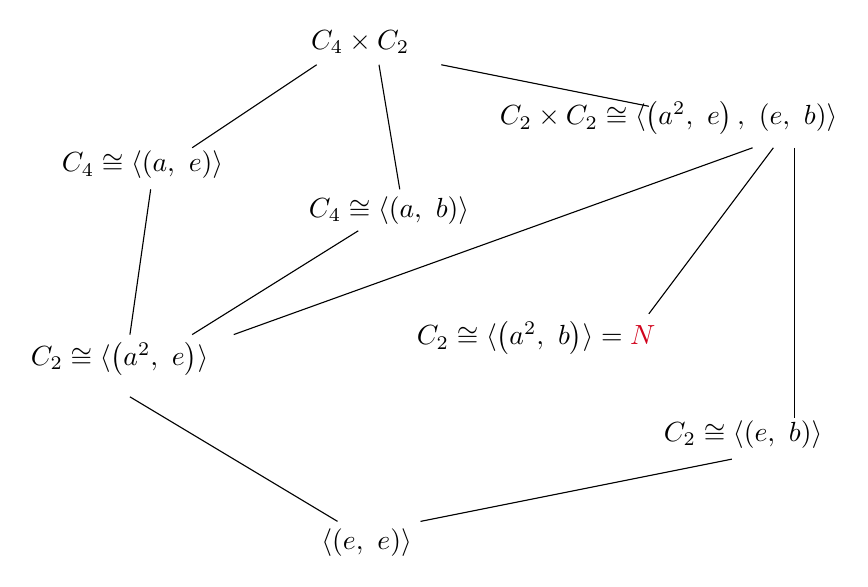
\begin{tikzpicture}[x=0.75pt,y=0.75pt,yscale=-1,xscale=1]
%uncomment if require: \path (0,300); %set diagram left start at 0, and has height of 300

%Straight Lines [id:da3052798466082476] 
\draw    (80,170) -- (90,100) ;
%Straight Lines [id:da6277397655458354] 
\draw    (170,40) -- (110,80) ;
%Straight Lines [id:da15377901054267062] 
\draw    (180,260) -- (80,200) ;
%Straight Lines [id:da1699584070636042] 
\draw    (370,230) -- (220,260) ;
%Straight Lines [id:da1875896852440162] 
\draw    (200,40) -- (210,100) ;
%Straight Lines [id:da13929797547891787] 
\draw    (190,120) -- (110,170) ;
%Straight Lines [id:da757023270257581] 
\draw    (230,40) -- (330,60) ;
%Straight Lines [id:da3738137975747218] 
\draw    (400,80) -- (400,210) ;
%Straight Lines [id:da9092849551708699] 
\draw    (380,80) -- (130,170) ;
%Straight Lines [id:da0785484493397397] 
\draw    (390,80) -- (330,160) ;

% Text Node
\draw (46,80.4) node [anchor=north west][inner sep=0.75pt]    {$C_{4} \cong \langle ( a,\ e) \rangle $};
% Text Node
\draw (166,22.4) node [anchor=north west][inner sep=0.75pt]    {$C_{4} \times C_{2}$};
% Text Node
\draw (31,172.4) node [anchor=north west][inner sep=0.75pt]    {$C_{2} \cong \langle \left( a^{2} ,\ e\right) \rangle $};
% Text Node
\draw (165,102.4) node [anchor=north west][inner sep=0.75pt]    {$C_{4} \cong \langle ( a,\ b) \rangle $};
% Text Node
\draw (171,262.4) node [anchor=north west][inner sep=0.75pt]    {$\langle ( e,\ e) \rangle $};
% Text Node
\draw (217,162.4) node [anchor=north west][inner sep=0.75pt]    {$C_{2} \cong \langle \left( a^{2} ,\ b\right) \rangle =\textcolor[rgb]{0.82,0.01,0.11}{N}$};
% Text Node
\draw (336,210.4) node [anchor=north west][inner sep=0.75pt]    {$C_{2} \cong \langle ( e,\ b) \rangle $};
% Text Node
\draw (257,56.4) node [anchor=north west][inner sep=0.75pt]    {$C_{2} \times C_{2} \cong \langle \left( a^{2} ,\ e\right) ,\ ( e,\ b) \rangle $};


\end{tikzpicture}
	\end{center}
	We will define $N = \langle (a^2, b) \rangle$, which is normal because our group is abelian. Then if we look at $C_4 \times C_2 / N$, then the correspondence theorem tells us that it's subgroups are the intermediate subgroups between $C_4 \times C_2$ and $N$, and thus it has the following subgroup lattice.
	\begin{center}
		

\tikzset{every picture/.style={line width=0.75pt}} %set default line width to 0.75pt        

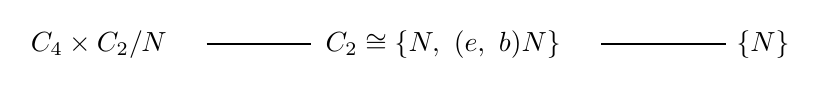
\begin{tikzpicture}[x=0.75pt,y=0.75pt,yscale=-1,xscale=1]
%uncomment if require: \path (0,300); %set diagram left start at 0, and has height of 300

%Straight Lines [id:da6524934164402587] 
\draw    (167,30) -- (217,30) ;
%Straight Lines [id:da3488573500514882] 
\draw    (357,30) -- (417,30) ;

% Text Node
\draw (81,22.4) node [anchor=north west][inner sep=0.75pt]    {$C_{4} \times C_{2} /N$};
% Text Node
\draw (223,22.4) node [anchor=north west][inner sep=0.75pt]    {$C_{2} \cong \{N,\ ( e,\ b) N\}$};
% Text Node
\draw (421,22.4) node [anchor=north west][inner sep=0.75pt]    {$\{N\}$};


\end{tikzpicture}

	\end{center}
	This also shows us that because $C_4 \times C_2 / N$ has order 4 by Lagrange, it must be isomorphic to $C_4$ (as otherwise it would be isomorphic to $C_2 \times C_2$, which would have a different subgroup lattice).
\end{example}

Now, if we had some subgroup $H \leq G$ that didn't contain $N \normal G$, we can still make a normal subgroup of $H$ by intersecting. This is the second isomorphism theorem.

\begin{theorem}[Second Isomorphism Theorem]
	Let $H \leq G$ and $N \normal G$. Then $H \cap N \normal H$ and $H/(H \cap N) \cong HN / N$.
\end{theorem}
\begin{proof}[Proof Sketch]
	When $N \normal G$ and $H \leq G$, then $HN = \{ hn : h \in H, n \in N\}$ is a subgroup of $H$, and $HN = \langle H, N \rangle$ (the smallest subgroups of $G$ containing $H$ and $N$). Then consider the function $\phi : H \rightarrow HN/N$, with $\phi(h) = hN$. We can check this is a well defined, surjective homomorphism, and it's kernel is $N \cap H$, and we can apply the first isomorphism to get $H/(N \cap H) \cong HN/N \leq G/N$.
\end{proof}

We mentioned previously that normality is preserved. We can even say something about quotients.

\begin{theorem}[Third Isomorphism Theorem]
	Let $N \leq M \leq G$ such that $N \normal G$ and $M \normal G$. Then $M/N \normal G/N$ and $(G/N) / (M/N) \cong G/M$.
\end{theorem}
\begin{proof}
	We define $\phi: G/N \rightarrow G/M$ by $\phi(gN) = gM$. $\phi$ is well-defined since $N \leq M$, and it's a surjective homomorphism. It's kernel is $M/N$, and thus by the first isomorphism theorem, $(G/N) / (M/N) \cong G/M$.
\end{proof}


Let's have a look at some examples of the isomorphism theorems.

\begin{example}
	Consider the group $\Z$, and define $H = 3\Z$ and $N = 5\Z$. Note that 
	Then by the second isomorphism theorem as , $H/(H \cap N) \cong HN/N \cong \Z/5\Z$, as $\langle H, N \rangle = \Z$ by Bezout's lemma.
\end{example}


\section{Simple Groups}

We will finish this chapter with the introduction of \emph{simple groups}.

\begin{definition}[Simple Groups]
	A group $G$ is \vocab{simple} if its only normal subgroups are $\{e\}$ and $G$.
\end{definition}

\begin{example}[Examples of Simple Groups]
The following are simple groups:
\begin{itemize}
	\item $C_p$ for a prime $p$.
	\item $A_5$ (we will prove this later on).
\end{itemize}	
\end{example}

Finite simple groups are important as they can be thought of as the `building blocks' of all finite groups. If we have some finite group with a normal subgroup, we can take the quotient by that normal subgroup, and you would obtain two objects (the quotient and the normal subgroup) that are smaller than the original group. These objects can help you understand the groups more, but simple groups can't be decomposed further.

Recently, the classification of all finite simple groups was completed, and you can find a large book with all finite simple groups in it!

\chapter{Group Actions}

The next aspect of group theory we shall look at is \emph{group actions}, where we study how groups interact with other objects. This isn't such a foreign concept -- if you consider the examples of groups that we have looked at previously, we have in many cases been able to identify elements by their effect on some set. For example, we determined the elements of $S_n$ by how it permuted elements of the set $\{1, 2, \dots, n\}$, and we defined $D_{2n}$ based on the symmetries of an $n$-gon.

Of course, using the group axioms we can somewhat forget that these were ever groups that acted on certain objects, but by introducing these objects that groups can act upon adds a certain richness to the subject.

\begin{definition}[Group Action]
Let $G$ be a group, and let $X$ be a set. An \vocab{action} of $G$ on $X$ is a function $\alpha : G \times X \rightarrow X$ written $\alpha(g, x) = \alpha_g(x)$, satisfying
\begin{itemize}
	\item $\alpha_g(x) \in X$ for all $g \in G$ and $x \in X$.
	\item $\alpha_e(x) = x$ for all $x \in X$.
	\item $\alpha_g \circ \alpha_h (x) = \alpha_{gh}(x)$ for any $g, h \in G$ and $x \in X$.
\end{itemize}
\end{definition}

\begin{example}
The following are all examples of groups that act on various sets.
\begin{enumerate}[label=(\roman*)]
	\item The group $S_n$ acts on $X$ by permutation.
	\item The group $D_{2n}$ acts on the vertices of a regular $n$-gon, and if we label these vertices 1, 2, $\dots$, $n$, we get an action on the set $\{1, 2, \dots, n\}$.
	\item The group $D_{2n}$ acts on the vectices of a regular $n$-gon, and if we label these vertices 1, 2, $\dots$, $n$, we get an action on the set $\{1, 2, \dots, n\}$.
	\item The symmetries of a cube act on a set of vertices, a set of edges, a set of faces, and a set of pairs of opposite faces.
\end{enumerate}
\end{example}

\begin{remark}
	These examples show us that more than one group can act on a given set, for example in (i) and (ii). A group can also act on many sets.
\end{remark}

\begin{lemma}\label{lemma:bijection}
	For all $g \in G$ and an action $\alpha_g: X \rightarrow X$, the map $x \mapsto \alpha_g(x)$ is a bijection.
\end{lemma}
\begin{proof}
	We have $\alpha_g(\alpha_{g^{-1}}(x)) = \alpha_{g g^{-1}}(x) = \alpha_e(x) = x$ for all $x \in X$, and similarily, $\alpha_{g^{-1}}(\alpha_g(x)) = x$ for all $x \in X$. Hence $\alpha_g \circ \alpha_{g^{-1}}$ and $\alpha_{g^{-1}} \circ \alpha_{g}$ are the identity functions, so $\alpha_g$ is a bijection.
\end{proof}

We can also define actions by linking $G$ to $\sym(X)$ in the following way.

\begin{proposition}
	Let $G$ be a group, and $X$ be a set. Then $\alpha: G \times X \rightarrow X$ is an action if and only if the function $\rho: G \rightarrow \sym(X)$ where $\rho(g) = \alpha(g)$ is a homomorphism.
\end{proposition}
\begin{proof}
	If $\alpha$ is an action, then by \autoref{lemma:bijection}, $\alpha_g$ is a bijection from $X \rightarrow X$, so $\alpha_g \in \sym(X)$. Now $\rho(gh) = \alpha_{gh}$ and for all $x \in X$, $\alpha_{gh}(x) = \alpha_g \circ \alpha_h (x)$, so $\rho(gh) = \alpha_{gh} = \alpha_g \circ \alpha_h = \rho(g) \rho(h)$, so $\rho$ is a homomorphism.

	Otherwise, if we have some homomorphism $\rho : G \rightarrow \sym(X)$, we can define $\alpha: G \times X \rightarrow X$ by $\alpha(g, x) = \alpha_g(x)  = \rho(g)(x)$. Then $\alpha$ is an action. This is true because $\rho(g) \in \sym(X)$, so $\rho(g)(x) = \alpha_g(x) \in X$, and $\rho(e)$ is the identity in $\sym(X)$ which implies $\rho(e)(x) = x$, and finally, $\rho(gh) = \rho(g) \rho(h)$ implies that $\alpha_{gh}(x) = \alpha_g \circ \alpha_g (x)$ for all $x \in X$.   
\end{proof}

We can make the notation slightly easier. When we write $\alpha_g : X \rightarrow X$, we can really think of $g$ as being a function on $x$, and we can write $g(x)$ instead.

With the above proposition in mind, we can define the \emph{kernel} of an action.

\begin{definition}
	The \vocab{kernel of an action} $\alpha : G \times X \rightarrow X$ is the kernel of the homomorphism $\rho : G \rightarrow \sym(x)$ (as above).
\end{definition}
These are all of the elements of $G$ that act as the identity of $\sym(X)$, that is, they do nothing to every $x \in X$. Note that by the first isomorphism theorem, this also implies that $G/\kernel \rho \cong \image \rho \leq \sym(X)$, and thus if $\kernel \rho = \{e\}$, then $G \leq \sym(X)$.

\begin{example}~
	    \vspace*{-1.5\baselineskip}
	\begin{enumerate}[label=(\roman*)]
		\item $D_{2n}$ acting on $\{1, \dots, n\}$ (the labelled vertices on an $n$-gon) has $\kernel \rho = \{ e\}$, as every non-trivial element of $D_{2n}$ moves at least one vertex. Thus $D_{2n} \leq S_n$.
		\item Let $G$ be the symmetries of a cube, and consider $X$ to be the set of unordered pairs of opposite faces. Then $|X| = 3$. So we get a homomorphism $\rho : G \rightarrow S_3$. Clearly there are symmetries of the cube that realize all of the permutation of $X$, so $\rho$ is surjective. So, $G/\kernel \phi \cong S_3$.
	\end{enumerate}
\end{example}

\begin{definition}[Faithful Actions]
	An action of $G$ on $X$ is called \vocab{faithful} if $\ker \rho = \{ e\}$.
\end{definition}

\section{Orbits and Stabilisers}

Consider the following two questions: for a group $G$ acting on a set $X$, what elements of $X$ we can `get to' from a certain $x \in X$ using the action of $G$? Also, which group elements leave a given $x \in X$ unchanged? 

\clearpage
\chapter*{Biblography}

TODO: Make this proper.

\begin{itemize}
	\item Napkin by Evan Chen -- Used for a good few of the examples
	\item Abstract Algebra by Dummit and Foote -- General Reference
	\item Undergraduate Algebra, Serge Lang -- Genereal Reference
	\item A Book of Abstract Algebra, Charles Pinter -- General Reference and used in the development of Quotient Groups
	\item Dexter Chua and David Bai's notes -- For a general view on the course structure before the lectures were completed, along with some of the proofs that were omitted from our lectures.
\end{itemize}

\end{document}
